% Options for packages loaded elsewhere
\PassOptionsToPackage{unicode}{hyperref}
\PassOptionsToPackage{hyphens}{url}
%
\documentclass[
  12pt,
]{article}
\usepackage{amsmath,amssymb}
\usepackage{lmodern}
\usepackage{iftex}
\ifPDFTeX
  \usepackage[T1]{fontenc}
  \usepackage[utf8]{inputenc}
  \usepackage{textcomp} % provide euro and other symbols
\else % if luatex or xetex
  \usepackage{unicode-math}
  \defaultfontfeatures{Scale=MatchLowercase}
  \defaultfontfeatures[\rmfamily]{Ligatures=TeX,Scale=1}
\fi
% Use upquote if available, for straight quotes in verbatim environments
\IfFileExists{upquote.sty}{\usepackage{upquote}}{}
\IfFileExists{microtype.sty}{% use microtype if available
  \usepackage[]{microtype}
  \UseMicrotypeSet[protrusion]{basicmath} % disable protrusion for tt fonts
}{}
\makeatletter
\@ifundefined{KOMAClassName}{% if non-KOMA class
  \IfFileExists{parskip.sty}{%
    \usepackage{parskip}
  }{% else
    \setlength{\parindent}{0pt}
    \setlength{\parskip}{6pt plus 2pt minus 1pt}}
}{% if KOMA class
  \KOMAoptions{parskip=half}}
\makeatother
\usepackage{xcolor}
\IfFileExists{xurl.sty}{\usepackage{xurl}}{} % add URL line breaks if available
\IfFileExists{bookmark.sty}{\usepackage{bookmark}}{\usepackage{hyperref}}
\hypersetup{
  pdftitle={Estimation of survey efficiency and biomass for commercially important species from industry-based paired gear experiments},
  pdfauthor={Timothy J. Miller1,2; David E. Richardson3; Philip J. Politis2; Christopher D. Roebuck4; John P. Manderson5,6; Michael H. Martin2,7; Andrew W. Jones3},
  hidelinks,
  pdfcreator={LaTeX via pandoc}}
\urlstyle{same} % disable monospaced font for URLs
\usepackage[margin=1in]{geometry}
\usepackage{graphicx}
\makeatletter
\def\maxwidth{\ifdim\Gin@nat@width>\linewidth\linewidth\else\Gin@nat@width\fi}
\def\maxheight{\ifdim\Gin@nat@height>\textheight\textheight\else\Gin@nat@height\fi}
\makeatother
% Scale images if necessary, so that they will not overflow the page
% margins by default, and it is still possible to overwrite the defaults
% using explicit options in \includegraphics[width, height, ...]{}
\setkeys{Gin}{width=\maxwidth,height=\maxheight,keepaspectratio}
% Set default figure placement to htbp
\makeatletter
\def\fps@figure{htbp}
\makeatother
\setlength{\emergencystretch}{3em} % prevent overfull lines
\providecommand{\tightlist}{%
  \setlength{\itemsep}{0pt}\setlength{\parskip}{0pt}}
\setcounter{secnumdepth}{5}
\newlength{\cslhangindent}
\setlength{\cslhangindent}{1.5em}
\newlength{\csllabelwidth}
\setlength{\csllabelwidth}{3em}
\newlength{\cslentryspacingunit} % times entry-spacing
\setlength{\cslentryspacingunit}{\parskip}
\newenvironment{CSLReferences}[2] % #1 hanging-ident, #2 entry spacing
 {% don't indent paragraphs
  \setlength{\parindent}{0pt}
  % turn on hanging indent if param 1 is 1
  \ifodd #1
  \let\oldpar\par
  \def\par{\hangindent=\cslhangindent\oldpar}
  \fi
  % set entry spacing
  \setlength{\parskip}{#2\cslentryspacingunit}
 }%
 {}
\usepackage{calc}
\newcommand{\CSLBlock}[1]{#1\hfill\break}
\newcommand{\CSLLeftMargin}[1]{\parbox[t]{\csllabelwidth}{#1}}
\newcommand{\CSLRightInline}[1]{\parbox[t]{\linewidth - \csllabelwidth}{#1}\break}
\newcommand{\CSLIndent}[1]{\hspace{\cslhangindent}#1}
\usepackage{url}
\usepackage{setspace}
%\singlespacing
%\onehalfspacing
\doublespacing
\usepackage{lineno}
\linenumbers
\usepackage[belowskip=0pt,aboveskip=0pt]{caption}
\usepackage{relsize}
\newcommand{\afrb}{Alaska Fishery Research Bulletin\xspace}
\newcommand{\ajms}{African Journal of Marine Science\xspace}
\newcommand{\amb}{Advances in Marine Biology\xspace}
\newcommand{\bms}{Bulletin of Marine Science\xspace}
\newcommand{\bjssf}{Bulletin of the Japanese Society of Scientific Fisheries\xspace}
\newcommand{\cb}{Conservation Biology\xspace}
\newcommand{\cjfas}{Canadian Journal of Fisheries and Aquatic Sciences\xspace}
\newcommand{\ea}{Ecological Applications\xspace}
\newcommand{\eer}{Evolutionary Ecology Research\xspace}
\newcommand{\elet}{Ecology Letters\xspace}
\newcommand{\emod}{Ecological Modelling\xspace}
\newcommand{\ebf}{Environmental Biology of Fishes\xspace}
\newcommand{\ff}{Fish and Fisheries\xspace}
\newcommand{\fo}{Fisheries Oceanography\xspace}
\newcommand{\fr}{Fisheries Research\xspace}
\newcommand{\fb}{Fishery Bulletin\xspace}
\newcommand{\ijms}{ICES Journal of Marine Science\xspace}
\newcommand{\iccat}{Collective Volume of Scientific Papers ICCAT\xspace}
\newcommand{\jae}{Journal of Animal Ecology\xspace}
\newcommand{\jai}{Journal of Applied Ichthyology\xspace}
\newcommand{\jdc}{Journal Du Conseil International Pour L'exploration De La Mer\xspace}
\newcommand{\jdcp}{Journal Du Conseil Permanent International Pour L'exploration De La Mer\xspace}
\newcommand{\jembe}{Journal of Experimental Marine Biology and Ecology\xspace}
\newcommand{\jfb}{Journal of Fish Biology\xspace}
\newcommand{\jsr}{Journal of Sea Research\xspace}
\newcommand{\jtb}{Journal of Theoretical Biology\xspace}
\newcommand{\jfrbc}{Journal of the Fisheries Research Board of Canada\xspace}
\newcommand{\jnwafs}{Journal of Northwest Atlantic Fisheries Science\xspace}
\newcommand{\mcf}{Marine and Coastal Fisheries: Dynamics, Management, and Ecosystem Science\xspace}
\newcommand{\mb}{Marine Biology\xspace}
\newcommand{\meps}{Marine Ecology Progress Series\xspace}
\newcommand{\mfr}{Marine Fisheries Review\xspace}
\newcommand{\mpb}{Marine Pollution Bulletin\xspace}
\newcommand{\najfm}{North American Journal of Fisheries Management\xspace}
\newcommand{\nzjmfr}{New Zealand Journal of Marine and Freshwater Research\xspace}
\newcommand{\pnas}{Proceedings of the National Academy of Sciences USA\xspace}
\newcommand{\rpvrciemm}{Rapports et Proc\`es-Verbaux des R\'eunions. Conseil Internationale pour l'Exploration de la Mer\xspace}
\newcommand{\rpvrcpiemm}{Rapports et Proc\`es-Verbaux des R\'eunions. Conseil Permanent Internationale pour l'Exploration de la Mer\xspace}
\newcommand{\rfbf}{Reviews in Fish Biology and Fisheries\xspace}
\newcommand{\sajms}{South African Journal of Marine Science\xspace}
\newcommand{\tafs}{Transactions of the American Fisheries Society\xspace}

\newcommand{\anzjs}{Australian \& New Zealand Journal of Statistics\xspace}
\newcommand{\as}{Applied Statistics\xspace}
\newcommand{\csda}{Computational Statistics \& Data Analysis\xspace}
\newcommand{\ees}{Environmental and Ecological Statistics\xspace}
\newcommand{\jas}{Journal of Applied Statistics\xspace}
\newcommand{\jabes}{Journal of Agricultural, Biological, and Environmental Statistics\xspace}
\newcommand{\jasa}{Journal of the American Statistical Association\xspace}
\newcommand{\jrssb}{Journal of the Royal Statistical Society. Series B\xspace}
\newcommand{\sm}{Statistics in Medicine}

\usepackage{xspace}
\usepackage{bm}
\usepackage{caption,graphics}
\usepackage{graphicx}
\usepackage{makecell}
\renewcommand\figurename{Fig.}
\captionsetup{labelsep=period, singlelinecheck=false}
\newcommand{\changesize}[1]{\fontsize{#1pt}{#1pt}\selectfont}
\renewcommand{\arraystretch}{1.5}
\renewcommand\theadfont{}
\usepackage{booktabs}
\usepackage{longtable}
\usepackage{array}
\usepackage{multirow}
\usepackage{wrapfig}
\usepackage{float}
\usepackage{colortbl}
\usepackage{pdflscape}
\usepackage{tabu}
\usepackage{threeparttable}
\usepackage{threeparttablex}
\usepackage[normalem]{ulem}
\usepackage{makecell}
\usepackage{xcolor}
\ifLuaTeX
  \usepackage{selnolig}  % disable illegal ligatures
\fi
\usepackage[]{natbib}
\bibliographystyle{cjfas2.bst}

\title{Estimation of survey efficiency and biomass for commercially
important species from industry-based paired gear experiments}
\author{Timothy J. Miller\textsuperscript{1,2} \and David E.
Richardson\textsuperscript{3} \and Philip J.
Politis\textsuperscript{2} \and Christopher D.
Roebuck\textsuperscript{4} \and John P.
Manderson\textsuperscript{5,6} \and Michael H.
Martin\textsuperscript{2,7} \and Andrew W. Jones\textsuperscript{3}}
\date{}

\begin{document}
\maketitle

\(^1\)corresponding author:
\href{mailto:timothy.j.miller@noaa.gov}{\nolinkurl{timothy.j.miller@noaa.gov}}\\
\(^2\)Northeast Fisheries Science Center, Woods Hole Laboratory, 166
Water Street, Woods Hole, MA 02543 USA\\
\(^3\)Northeast Fisheries Science Center, Narragansett Laboratory, 28
Tarzwell Drive Narragansett, RI 02882 USA\\
\(^4\)Fishing Vessel Karen Elizabeth, Narragansett, RI 02882, USA\\
\(^5\)Northeast Fisheries Science Center, James J. Howard Marine
Sciences Laboratory, 74 Magruder Road Highlands, NJ 07732 USA\\
\(^6\)Current address: OpenOcean Research, Suite 101, 40 West Evergreen
Avenue, Philadelphia, PA, 19118 USA\\
\(^7\)Current address: Alaska Fisheries Science Center, 7600 Sand Point
Way N.E., Building 4 Seattle, WA 98115 USA

\pagebreak

\hypertarget{abstract}{%
\subsection*{Abstract}\label{abstract}}
\addcontentsline{toc}{subsection}{Abstract}

Fishery-independent surveys provide valuable information about trends in
population abundance for management of commercially important fish
stocks. A critical component of the relationship of the catches of the
survey to the size of a fish stock is the catch efficiency of the survey
gear. Using a general hierarchical model we estimated the relative
efficiency of a chain sweep to the rockhopper sweep used by the
Northeast Fisheries Science Center bottom trawl survey from paired-gear
experimental tows carried out between 2015 and 2017 using a twin-trawl
vessel. For 10 commercially important species, we fitted and compared a
set of models with alternative assumptions about variation of relative
efficiency between paired gear tows, size and diel effects on the
relative efficiency, and extra-binomial variation of observations within
paired gear tows. These analyses provided evidence of changes in
relative efficiency with size for all species and diel effects were
important for all but one species. We then used the bottom trawl survey
data from surveys between 2009 and 2019 with the relative catch
efficiency estimates from the best performing models to estimate annual
and seasonal chain sweep-based swept area biomass for 17 managed stocks.
We estimated uncertainty in all results using bootstrap procedures for
each data component. We also assessed the effect of calibration on
uncertainty and correlation of the annual biomass estimates.

\hypertarget{keywords}{%
\subsubsection*{Keywords}\label{keywords}}
\addcontentsline{toc}{subsubsection}{Keywords}

gear efficiency, biomass estimation, hierarchical generalized additive
models

\pagebreak

\hypertarget{introduction}{%
\section{Introduction}\label{introduction}}

Ecosystem monitoring surveys such as fisheries-independent trawl surveys
are used to obtain information on a range of species and are therefore
not optimized with respect to sampling design or gear for any one
species \citep{bijleveldetal12, wangetal18}. Gear and sampling protocols
are designed to provide consistent and representative samples that allow
indices of abundance at size and age to be developed for a suite of
species \citep{azarovitz81, thiessetal18}. To provide indices of
population abundance with minimal potential sources of bias, survey
bottom trawl gear must be configured to be towed across as wide a
variety of habitats as possible, including seafloor habitats with
complex physical structures.

Indices of abundance at age and size derived from fishery-independent
bottom trawl surveys are scaled to population size by the survey
catchability (\(q\)) parameter \citep{arreguinsanchez96}. Catchability
is typically estimated internally within stock assessment models that
incorporate fisheries landings, indices of abundance, and life history
parameters. However, the amount or quality of data and degree of
contrast in the time series is often such that this parameter, and
therefore the population size, is difficult to estimate
\citep{maunderpiner15}. In such cases, estimates of survey catchability
from auxiliary data can inform the stock assessment. These external
estimates can be used as a direct input into the assessment model
\citep{somertonetal99}, can serve as a diagnostic measure of model
accuracy \citep{milleretal19}, or contribute to an alternate means of
providing catch advice when an assessment model is not considered
acceptable \citep{legaultmccurdy17}.

Catchability can be decomposed into two components, the proportion of
the population available to the survey sampling frame and the efficiency
of the survey gear given an individual is available to the gear
\citep{paloheimodickie64}. Here efficiency is the fraction of available
fish retained by the gear, equivalent to availability-selection in
\citet{millarfryer99}. Estimates of these components allow relative
abundance indices to be converted into absolute abundance indices
without a population model. As such, investigations of gear mensuration
\citep{kotwickietal11}, species-specific gear efficiency
\citep{thygesenetal19}, and availability of the stock to the survey
design frame \citep{nicholetal19} improve our understanding of
catchability and therefore abundance of fish stocks.

Paired-gear studies where two gears are fished either concurrently or
close together temporally and spatially have long been used to estimate
the efficiency of one fishing gear relative to another
\citep[e.g.,][]{gulland64,bourne65}. Of the two gears, one is often a
reference gear that may be a gear currently used for annual surveys
\citep[e.g.,][]{munrosomerton01}. Typically neither of the gears is
fully efficient and therefore the relative efficiency of gears is
estimated \citep[e.g.,][]{miller13,kotwickietal17}, but there are cases
where one of the gears is assumed to be very nearly fully efficient
\citep[e.g.,][]{somertonetal13, milleretal19}.

Whether or not full efficiency of one of the gears is assumed,
paired-gear studies are essential for generating abundance time series
from fishery-independent surveys when there are changes in the vessel
and(or) gears over time due to gear failures or improved technology
\citep{pelletier98}. These studies are also helpful for combining
surveys conducted close together in space or time using alternative
gears \citep{kotwickietal13}.

Within the northeast US there has been a heightened focus on bottom
trawl survey operations and gear efficiency. To help provide clarity on
the trawl operations and build trust in survey indices the New England
and Mid-Atlantic Fisheries Management Councils developed a Northeast
Trawl Advisory Panel. This panel is composed of members from industry,
regional academics, as well as state and federal scientists. Together
the group designed a set of experiments to better understand the
efficiency of the bottom trawl survey gear for northeast US groundfish
stocks.

In conducting paired-gear studies it is ideal to have the two gears
deployed as close together spatially and temporally as possible to
reduce variation between the gears in densities of the species being
encountered. The twin-trawl rigging \citep{kragetal15} where two trawls
can be fished simultaneously approaches this ideal \citep{ices96}, and
is the data-collection platform chosen by the Trawl Advisory Panel. The
Panel decided to rig one of the twin trawls as the the gear used by the
bottom trawl survey which uses a rockhopper sweep. The Trawl Advisory
Panel decided to focus the experiments on efficiency for flatfishes, so
the other trawl was rigged similarly except with a chain sweep in an
attempt to eliminate any escapement of fish under the gear. The Panel
thought that a chain sweep would limit escapement under the sweep better
than a flat or cookie sweep or other potential sweep designs. The sweep
was constructed of multiple layers of chain so as to maximize bottom
contact and minimize loss but also reduce retaining debris in the net
and the trawl hanging on obstructions. If the chain sweep-based gear is
assumed to be fully efficient, the efficiency of the rockhopper
sweep-based gear used by the bottom trawl survey can be estimated from
these experiments.

The analytical methods to estimate the efficiency of the bottom trawl
gear are based on those used by \citet{miller13} to estimate size
effects on relative catch efficiency of the NOAA Ship \emph{Henry B.
Bigelow} (\emph{Bigelow}) to the NOAA Ship \emph{Albatross IV} for a
variety of commercially important species. We extend the model to
consider different size effects for tows conducted during the day or
night since both the spring and fall bottom trawl surveys conducted in
the Northeast US are 24-hour operations. We apply these methods to
paired gear observations and estimate relative efficiency of the chain
sweep and rockhopper sweep gears. We also apply the estimated efficiency
of the rockhopper gear to survey data to estimate spring and fall
biomass indices from 2009-2019 for 17 commercially important fish stocks
in the Northeast US (Table \ref{stock_definition_table}).

The relative catch efficiency estimates provided by analyses of paired
gear data have uncertainty which may not be propagated when applied to
survey data to make estimates of abundance. The application to survey
data also induces correlation of the annual (and seasonal) abundance
estimates from these surveys. These indices are typically used as
measures of relative abundance in stock assessment with the precision of
the indices used to weight the observations within the assessment model
where the observations for each of the annual and seasonal indices is
typically assumed to be independent of the others. Here we compare the
precision of the biomass indices calibrated to the chain sweep gear to
that of the and uncalibrated indices using the rockhopper sweep gear and
measure the correlation of calibrated indices for each stock.

\hypertarget{methods}{%
\section{Methods}\label{methods}}

\hypertarget{data-collection}{%
\subsection{Data collection}\label{data-collection}}

Data were collected during three field experiments carried out in 2015,
2016, and 2017, respectively, aboard the \emph{F/V Karen Elizabeth}, a
23.8m (78ft) stern trawler capable of towing two trawls simultaneously
side by side (Figure \ref{twin_trawl_diagram}). One side of the
twin-trawl rig towed a NEFSC standard 400 x 12 cm survey bottom trawl
rigged with the NEFSC standard rockhopper sweep \citep{politisetal14}
(Figure \ref{twin_trawl_photo}). The other side of the twin-trawl rig
towed a modified version of the NEFSC 400 x 12cm survey bottom trawl
with the intent of altering design characteristics of the standard
survey trawl to improve bottom contact and maximize the capture of
flatfish. The modifications included reducing the headline flotation
from 66 to 32, 20cm, spherical floats, reducing the port and starboard
top wing-end extensions by 50cm each, and utilizing a chain sweep. The
chain sweep was constructed of 1.6cm (\(\frac{5}{8}\)in) trawl chain
covered by 12.7cm diameter x 1cm thick rubber discs on every other chain
link (Figure \ref{twin_trawl_photo}). Two rows of 1.3cm
(\(\frac{1}{2}\)in) tickler chains were attached to the 1.6cm trawl
chain by 1.3cm shackles. To ensure equivalent net geometry of each gear,
32m restrictor ropes, made of 1.4cm (\(\frac{9}{16}\)in) buoyant,
Polytron rope, were attached between each of the trawl doors and the
center clump. 3.4m\(^2\) Thyboron Type 4 trawl doors were used to
provide enough spreading force to ensure the restrictor ropes remained
taut throughout each tow. Each trawl used the NEFSC standard 36.6m
bridles. Every tow was monitored with net mensuration sensors to verify
bridals were held to optimal angles and identical spread. All tows
followed the NEFSC standard survey towing protocols of 20 minutes at 3.0
knots. Port and starboard net spreads were measured separately with two
sets of Simrad ITI acoustic net mensuration sensors measuring from the
port wing-end to the center clump and the starboard wing-end to the
center clump. In 2015, 108 (45 day, 63 night) paired tows were conducted
in eastern Georges Bank and off of southern New England (Figure
\ref{tow_locations}). In 2016, 117 (74 day, 43 night) paired tows were
conducted in western Gulf of Maine and the northern edge of Georges
Bank. In 2017, 103 (61 day, 42 night) paired tows were conducted in the
western Gulf of Maine and off of southern New England. Paired tows were
denoted as ``day'' and ``night'' by whether the sun was above or below
the horizon at the time of the tow.

In order to reduce shipboard processing time and maximize the number of
tows, only select taxa were enumerated and measured for total length,
rather than the full processing of all species as occurs on the trawl
survey \citep{politisetal14}. All flatfish species (order
Pleuronectiformes), thorny skate (\emph{Amblyraja radiata}), barndoor
skate (\emph{Dipturus laevis}) and goosefish (\emph{Lophias americanus})
collected in each net of each tow were independently sorted, weighed and
measured in all years. If the catch of a species was greater than
\({\approx}150\) individuals, a subsample of \({\approx}150\)
individuals was measured. Red hake (\emph{Urophycis chuss}) were not
quantified during the 2015 and 2016 sampling because other species were
prioritized, but were fully processed in 2017. Winter skate
(\emph{Leucoraja ocellata}) and little skate (\emph{L. erinacea}) were
weighed in all years and but were not separated to species nor measured.
Sea scallops were weighed in 2015 and 2016, but not 2017.

\hypertarget{paired-tow-analysis}{%
\subsection{Paired-tow analysis}\label{paired-tow-analysis}}

We employed the hierarchical modeling approach from \citet{miller13} to
estimate the efficiency (\(\rho\)) of the rockhopper sweep used by the
NEFSC bottom trawl survey relative to the chain sweep-based gear for ten
species (Summer flounder, \emph{Paralichthys dentatus}; American plaice,
\emph{Hippoglossoides platessoides}; windowpane flounder,
\emph{Scophthalmus aquosus}; winter flounder, \emph{Pseudopleuronectes
americanus}; yellowtail flounder, \emph{Limanda ferruginea}; witch
flounder, \emph{Glyptocephalus cynoglossus}; red hake; goosefish;
barndoor skate; thorny skate) from the data collected during the three
trips carried out aboard the \emph{F/V Karen Elizabeth}. We first fit
and compared the same set of 13 models as \citet{miller13} with
different assumptions about variation of relative efficiency between
paired gear tows, size effects on the relative efficiency, and
extra-binomial variation of observations within paired gear tows. The
binomial (BI\(_0\) to BI\(_4\)) and beta-binomial (BB\(_0\) to BB\(_7\))
models that were fitted for all species are described in Table
\ref{base_model_description} including pseudo-formulas analogous to
those used to specify and fit mixed or generalized additive models in R
\citep{R19,wood06}. We then also included diel effects on relative catch
efficiency and interactions with size effects with the best performing
model of the original 13 models for each species. To fit these diel
effects, we generalized the modeling framework somewhat in that we
allowed multiple (cubic regression spline) smooth effects, differing by
day and night, on relative catch efficiency. We implemented the models
using the Template Model Builder package \citep{kristensenetal16} in R
and we used the ``nlminb'' optimizer to fit the models by maximizing the
Laplace approximation of the marginal likelihood \citep{R19}.

We assessed convergence of the optimization for each model in two ways.
The first criterion was whether the optimization using nlminb completed
without error. The errors for these models was due to entering the
parameter space where the gradient was not defined. Note that TMB uses
automatic differentiation to provide a gradient function for use in
optimization. The second convergence criterion was whether the flag
returned by nlminb indicated false convergence which is associated with
overparameterization of the model and that a simpler model (e.g., no
random effects or smoother) is warranted. Models that did not satisfy
these criteria were not considered further for relative performance
based on AIC. If the best performing model included smooth length
effects and the estimated smoothing parameter implied a linear functions
of length (on the transformed mean), then simple linear functions (i.e.,
completely smooth) were assumed for further models that included diel
effects on relative efficiency. As such, there was one less (smoothing)
parameter estimated for these models.

We compared two alternative ways of estimating uncertainty in relative
catch efficiency for the best performing models. The first estimation
approach uses the inverted hessian of the marginal log-likelihood and
the delta-method to estimate uncertainty in the predicted relative catch
efficiency at size. The second method is a bootstrap method where we
refit models to bootstrap resamples of the paired station data.
Specifically, we resampled the paired tows with replacement so that the
total number of paired tows was the same for a given species, but the
total number of length measurements varied depending on which of the
paired tows entered the sample for a particular bootstrap. We made 1000
bootstrap samples and estimated relative catch efficiency at size from
each bootstrap data set if the fitted model converged and the hessian at
the maximized log-likelihood was invertible.

For models BI\(_4\), BB\(_6\), and BB\(_7\), there are two fixed effects
parameters associated with the spline coefficients that are treated as
random effects for station-specific smoothers and the correlation of
these pairs of random effects is estimated. However, this parameter was
not estimable for red hake for BB\(_6\) and assumed equal to zero.

\hypertarget{length-weight-analysis}{%
\subsection{Length-weight analysis}\label{length-weight-analysis}}

We will use the relative catch efficiency at length to rescale the
abundance at length from the surveys. To generate a rescaled biomass
estimate, we convert the numbers at length to biomass at length using
estimates of weight at length and then sum across lengths. We fit
length-weight relationships to the length and weight observations for
each survey each year. We assumed weight observation \(j\) from survey
\(i\), was log-normal distributed, \begin{equation}\label{wal}
 \log W_{ij} \sim \text{N}\left(\log \alpha_i + \beta_i \log L_{ij} - \frac{\sigma_i^2}{2}, \sigma_i^2\right)
\end{equation} Because the expection of a log-normal random variable is
a function of the mean of the normal distribution and \(\sigma_i^2\), we
used a bias correction to ensure the expected weight
\(E(W_{ij})= \alpha_i L_{ij}^{\beta_i}\). We estimated parameters by
maximizing the model likelihood programmed with the Template Model
Builder package and R and generated predictions of weight at length
\begin{equation}\label{predwal}
\widehat W(L) = \widehat \alpha L^{\widehat \beta}.
\end{equation} Like the relative catch efficiency, we made bootstrap
predictions of weight at length by sampling with replacement the
length-weight observations within each annual survey and refitting the
length-weight relationship to each of the bootstrap data sets.

\hypertarget{biomass-estimation}{%
\subsection{Biomass estimation}\label{biomass-estimation}}

For the 17 managed stocks that are populations of the species in the
Northeast US where we have estimated relative efficiency, we estimated
stock biomass for each spring and fall annual survey assuming 100\%
efficiency of the chain sweep gear by scaling the survey tow
observations by the relative efficiency of the chain sweep and
rockhopper sweep gears. Summer and witch flounders, American plaice, and
barndoor and thorny skates are managed as single unit stocks, but there
are three stocks of winter and yellowtail flounders, and two stocks of
windowpane, red hake, and goosefish (Table
\ref{stock_definition_table}). First, the tow-specific catches at length
are rescaled, \begin{equation}\label{nal}
\widetilde N_{hi}\left(L\right) = N_{hi}\left(L\right)\widehat \rho_i\left(L\right)
\end{equation} where \(N_{hi}(L)\) is the number at length \(L\) in tow
\(i\) from stratum \(h\) and \(\widehat \rho_i\left(L\right)\) is the
relative efficiency of the chain sweep to rockhopper sweep at length
\(L\) estimated from the twin trawl observations that may depend on the
diel characteristic of tow \(i\) if that factor is in the best model
fitted to the twin-trawl observations. Note that we have omitted any
subscripts denoting the year or season.

The stratified abundance estimate is then calculated using the
design-based estimator, \begin{equation}\label{Nal_estimate}
 \widehat N(L) = \sum^H_{h=1} \frac{A_h}{an_h}\sum^{n_h}_{i=1} \widetilde N_{hi}(L)
\end{equation} where \(A_h\) is the area of stratum \(h\), \(a\) is the
average swept area of a survey station tow, and \(n_h\) is the number of
tows that were made in stratum \(h\). The corresponding biomass estimate
is then \begin{equation}\label{biomass_estimate}
 \widehat B = \sum^{n_L}_{l=1} \widehat N(L = l) \widehat W(L=l)
\end{equation} where \(\widehat W(L=l)\) is the predicted weight at
length (Eq. \ref{predwal}) from fitting length-weight observations
described above. Length is typically measured to the nearest cm so
\(n_L\) indicates the number of 1 cm length categories observed during
the survey.

We used the same criteria for survey station selection as those
currently used to estimate indices of abundance or biomass for
management of each stock. For Gulf of Maine winter flounder we also
restricted the size classes in each tow to those \(\geq\) 30 cm as the
biomass of the population over this threshold is currently used for
management of this stock. For some stocks there were certain years where
some but not all of the set of survey strata used to define indices of
abundances were sampled by the bottom trawl survey. In those years, the
average catch per unit area was expanded to all of the stock strata
proportionally to the areas of the sampled and unsampled strata. The
fall 2017 survey was extremely restricted because of vessel mechanical
failure and indices are not available for summer flounder, SNE-MA
windowpane, and SNE-MA yellowtail flounder.

To estimate uncertainty in biomass, we used bootstrap results for the
relative catch efficiency and weight at length estimates along with
bootstrap samples of the survey data. Bootstrap data sets for each of
the annual surveys respected the stratified random designs by resampling
with replacement within each stratum \citep{smith97}. For each of the
1000 combined bootstraps, survey observations for bootstrap \(b\) were
scaled with the corresponding bootstrap estimates of relative catch
efficiency and predicted weight at length, using Eqs. \ref{Nal_estimate}
and \ref{biomass_estimate}.

We also used the bootstraps to summarize other aspects of the biomass
estimates. First, we used the bootstraps to calculate the ratio of
calibrated and uncalibrated biomass for each spring and fall annual
survey, which is the implicit relative catch efficiency in terms of
biomass. The uncalibrated biomass estimate for bootstrap \(b\) uses the
same resampled survey data as the calibrated biomass estimate except
that the bootstrap for the relative catch efficiency is not used (i.e.,
\(\widehat \rho_i\left(L\right) = 1\) in Eq. \ref{nal}). We also used
the bootstraps to compare the coefficients of variation (CV) of the
calibrated and uncalibrated biomass estimates. The CV for an annual
biomass estimate for year \(y\) from either the spring or fall survey
was calculated as \[
\text{CV}\left(\widehat B_y\right) = \frac{\text{SD}\left(\widehat B_y\right)}{\overline{\widehat B}_y}
\] where \[
\text{SD}\left(\widehat B_y\right) = \sqrt{\frac{\sum_{b=1}^K \left(\widehat B_{y,b} - \overline{\widehat B}_y\right)^2}{K-1}},
\] \[
\overline{\widehat B}_y = \frac{\sum_{b=1}^K \widehat B_{y,b}}{K},
\] and \(K\) is the number of bootstraps.

For summer flounder it was necessary to omit one of the 1000 bootstraps
of relative catch efficiency at length due to an extremely large value
to which the standard deviation and mean of the bootstraps were
sensitive. Finally, just as the uncertainty in \(\rho\left(L\right)\)
affects the uncertainty in the calibrated abundance at length and
biomass estimates, it also induces correlation among the annual and
seasonal estimates because the same estimates are applied to all of
them. We calculated the correlation of annual biomass estimates for
years \(y\) and \(z\) using the bootstrap estimates of biomass \[
Cor\left(\widehat B_y, \widehat B_z\right) = \frac{Cov\left(\widehat B_y, \widehat B_z\right)}{\text{SD}\left(\widehat B_y\right)\text{SD}\left(\widehat B_z\right)}
\] where the covariance is \[
Cov\left(\widehat B_y, \widehat B_z\right) = \frac{\sum_{b=1}^K \left(\widehat B_{y,b} - \overline{\widehat B}_y\right)\left(\widehat B_{z,b} - \overline{\widehat B}_z\right)}{K-1}.
\] We summarized the relative precision of the calibrated and
uncalibrated biomass estimates as the average of the annual ratios of
the CVs for the calibrated and uncalibrated estimates \[
\frac{1}{n_y} \sum^{n_y}_{y = 1}\frac{CV\left(\widehat B\left(\rho\right)\right)}{CV\left(\widehat B\right)}.
\] We summarized the correlation of biomass estimates as the mean
correlation of all annual calibrated biomass estimates \[
\overline {Cor} = \frac{1}{n_y(n_y-1)/2} \sum_{y=2}^{n_y} \sum_{z=1}^{y} Cor\left(\widehat B_y, \widehat B_z\right).
\] All code and most data files to run the analysis and generate biomass
estimates are available at
\url{https://github.com/timjmiller/chainsweep_paper}.

\hypertarget{results}{%
\section{Results}\label{results}}

\hypertarget{paired-tow-observations}{%
\subsection{Paired-tow observations}\label{paired-tow-observations}}

In terms of paired tows and total numbers of fish, flatfish were the
best sampled species, but goosefish was observed in the most paired-tows
and red hake was one of the most prevalent in terms of total numbers
caught (Table \ref{data_table}). Witch flounder was the most prevalent
flatfish species caught while yellowtail flounder was the most
frequently observed flatfish in terms of paired tows. The proportion of
fish measured for length relative to the number caught varied across
species. All summer flounder, barndoor skate, and thorny skate that were
captured were measured. Subsampling occurred for all other species with
a high proportion (\textgreater97\%) measured for winter flounder and
goosefish, a moderate proportion (50-97\%) measured for American plaice,
windowpane flounder, and yellowtail flounder, and a low proportion
(\textless50\%) measured for witch flounder and red hake.

\hypertarget{relative-catch-efficiency}{%
\subsection{Relative catch efficiency}\label{relative-catch-efficiency}}

As measured by AIC, the best performing models for all 10 species
included size effects on the relative efficiency of the chain and
rockhopper sweep gears and between-pair variability in relative catch
efficiency (Table \ref{base_model_compare}). Extrabinomial variation
(i.e., beta-binomial) in relative catch efficiency at size within pairs
was also important for American plaice, yellowtail flounder, witch
flounder, red hake, and thorny skate. Model convergence was an issue for
all species, particularly for the most complex models with pair-specific
smooth functions of length (BI\(_4\)) and smooth effects of size on the
beta-binomial dispersion parameter (BB\(_3\),BB\(_5\), and BB\(_7\)).

Including diel effects on relative catch efficiency improved model
performance for all species except American plaice (Table
\ref{best_model_compare}). For those species with diel effects on
relative catch efficiency, the ratio of the efficiencies was generally
greater for daytime observations than those for nighttime tows, with the
exception of large winter flounder (Figure \ref{sp_rho_plot}). The
largest differences in efficiency was estimated for smaller barndoor
skate. For most of the species, the differences in efficiency between
the gears was generally greater for smaller individuals. The large
variability in the empirical estimates of the relative efficiency at
size for each paired tow is reflected in the variation in the posterior
smooth estimates of relative efficiency at size for each paired tow.

All 1000 bootstrap fits of the paired tow data converged with invertible
hessians at the optimized log-likelihood and provided estimates of
relative catch efficiency at size for summer, windowpane, and yellowtail
flounder, and red hake, goosefish, and thorny skate. All but 2 of the
bootstraps for winter flounder and 3 for barndoor skate provided
estimates of relative catch efficiency. For witch flounder, 817
bootstraps provided estimates and only 386 provided estimates for
American plaice. One bootstrap fit for summer flounder was excluded due
to an extremely high relative efficiency of the chain sweep gear which
impeded estimation of standard errors from the bootstrap fits.

Generally, where data are prevalent the bootstrap and hessian-based
confidence intervals are similar across all species. However, sometimes
substantially different perceptions of confidence ranges exist at the
extremes of the length range for particular species where there are
fewer data and asymptotic properties of estimators can be less
applicable.

\hypertarget{biomass-estimation-1}{%
\subsection{Biomass estimation}\label{biomass-estimation-1}}

Total biomass estimates calibrated to the chain sweep gear were variable
across years for most stocks and without strong trend (Figure
\ref{stock_biomass_plot}). However, declining trends exist for the
Georges Bank and southern New England-Mid-Atlantic yellowtail flounder
stocks and an increasing trend for northern goosefish. Biomass estimates
were greatest on average for northern red hake and least for Gulf of
Maine winter flounder, although this biomass estimate excludes fish less
than 30 cm in length. Fall and spring biomass estimates were similar in
scale for most stocks, except that southern New England winter flounder
and northern goosefish estimates were typically greater in the fall than
the spring.

The relative catch efficiency of the rockhopper and chan sweep gears in
terms of biomass varies across survey years and seasons due primarily to
differences in size composition, but also variation in estimated
length-weight relationship parameters (Figure
\ref{stock_biomass_efficiency_plot}). The efficiency of the bottom trawl
survey gear was greatest for the winter flounder stocks and American
plaice (0.6 to 0.9) and least for red hake, witch flounder, windowpane,
and yellowtail flounder stocks (0.2 to 0.4). Precision of the estimated
annual biomass efficiencies was lowest for Georges Bank winter flounder
and the skate stocks. For Gulf of Maine winter flounder, southern red
hake, and barndoor skate, the average fall biomass efficiencies were
typically greater than in the spring although the differences were small
relative to the confidence intervals.

Comparing the average of estimated coefficients of variation for annual
calibrated and uncalibrated biomass estimates showed large increases for
summer flounder in the fall (\(> 50\%\)), southern New England winter
flounder in the spring (77\%), Georges Bank winter flounder (more than
200\% for spring and fall), northern red hake (95\% for spring and 178\%
for fall), northern goosefish in the fall (93\%), and barndoor skate
(\(>100\%\) for both spring and fall) induced by the variability in the
estimation of the relative catch efficiency of the gears using chain and
rockhopper sweep gears (Table \ref{stock_cv_ratios}). The effect of
calibration on the precision of the biomass estimates was relatively
minor for other stocks.

We observed little correlation of annual biomass estimates induced by
the relative catch efficiency estimation for most of the stocks (Table
\ref{stock_mean_cor}). However, the biomass estimates were highly
correlated for George Bank winter flounder in the spring (65\%) and
barndoor skate (\(>70\%\) on average). Estimates for Georges Bank winter
flounder in the fall, both red hake stocks, northern goosefish, and
thorny skate were greater than 20\% on average.

\hypertarget{discussion}{%
\section{Discussion}\label{discussion}}

The data that we used to estimate bottom trawl survey catch efficiency
came from an experiment using a twin trawler and many of the standard
tow protocols for the NEFSC survey on the \emph{Bigelow}. The
experimental net used on one side of the twin trawl was the same as the
standard survey trawl used on the \emph{Bigelow} except that it
contained roughly half the number of floats and the sweep was modified
to optimize flatfish catch by minimizing the ability of flatfish to pass
under the net. The other side of the twin trawl was essentially
identical to the standard gear used on the \emph{Bigelow.} The towing of
the standard survey bottom trawl on the twin trawl experiment differed
in a few ways from its deployment on the spring and fall bottom trawl
surveys, but we believe that these differences did not have a
significant effect on the results. The use of larger doors and the
restrictor rope served to fix the net geometries which may be the
biggest source of variability in comparative trawl catches
\citep{jonesetal21}. This setup also allowed us to avoid many of the
potential problems due to the large differences in size of the
\emph{Bigelow} and the \emph{F/V Karen Elizabeth}. We do not suspect
that the use of the restrictor rope would influence flatfish behavior in
front of the trawl because flatfish have been shown to generally not
react to trawling induced stimuli until they are in very close proximity
or even contacted by the fishing gear \citep{ryeretal10}. The spread
data indicated that the restrictor rope remained taut throughout the
towing process (setting, towing, hauling back), so we believe it likely
that the restrictor rope was almost always at least 1m off the bottom.
Our concerns about potential effects of the restrictor rope on species
that spend more time off the ground (e.g., Atlantic cod, \emph{Gadus
morhua}) led us to exclude them from analyses.

Herding is a known phenomenon for flatfish and many other species when
certain types of gear are used
\citep{rammxiao95,somertonmunro01,somertonetal07,roseetal10}.
\citet{somertonmunro01} considered two factors of bridle herding effects
on efficiency. The first factor was the size of the bridle path where
the bridle is off the ground (\(W_\text{off}\)) and the second factor,
the herding efficiency (\(h\)) was the fraction of fish in the bridle
contact path moved into the path of the net. The former is a function of
gear design, and controllable, whereas the latter is a function of fish
behavior with regard to the bridle when it is in contact with the
substrate. The bridle configuration on the bottom trawl survey is
designed to minimize contact with the bottom and lack of abrasion of
painted bridles used during one of the twin trawler research trips
provided evidence of little or no bridle contact during the paired tow
experiments used to collect the data used in this study. Furthermore,
studies have consistently found that herding behavior occurred during
the daytime
\citep{glasswardle89,somertonmunro01,ryerbarnett06,bryanetal14,ryeretal10,deanetal21}
with some studies indicating high herding coefficients (\(h\)) along the
sections of the bridles in contact with the bottom. Studies that have
evaluated herding at night or in low light conditions did not find
evidence for a directional herding response
\citep{glasswardle89,ryerbarnett06,ryer08,ryeretal10}. The minimal
bridle contact with the substrate and the large fraction of nighttime
tows during the bottom trawl survey suggests flatfish herding is
unlikely to be an important factor in catch efficiency for net
spread-based swept area.

On the other hand, the biomass estimates assume that the chain sweep
gear is fully efficient, but it is likely at least some small fraction
of fish, that may depend on size, are not captured by the gear. Trawl
configurations such as that described by \citet{munrosomerton02} could
be used to quantify the efficiency of the chain sweep gear were
considered by the Trawl Advisory Panel, but were not used due to
concerns that the attached underbag could alter the performance of the
standard survey gear and inhibit the utility in calibrating the survey
indices. The biomass estimates also implicitly assume that the entire
stock is available to the bottom trawl survey, but many of these stocks
extend somewhat outside of the survey strata used to define the indices
throughout the year and(or) seasonally due to migration. If either of
these assumptions are incorrect this method of biomass estimation would
be negatively biased (expected value of biomass estimates would be lower
than the true value). However, estimation using the data from these
paired-gear studies and these assumptions is less biased than those made
without them.

Diurnal differences in behavior including hiding from predators at
higher light levels and occurring higher in the water column at night,
possibly for feeding, have been observed for flatfish species
\citep{hempel64,verheijendegroot67,burrowsetal94,burrowsgibson95,ellisetal97,hurstduffy05}.
Diurnal differences in reaction to trawl gear have also been observed,
with flatfish attempting to avoid gear by staying near the bottom during
daytime and moving off bottom during nighttime \citep{ryerbarnett06}. It
is not possible to distinguish these behaviors from paired tow studies
alone, but the greater relative catch efficiencies of the chain sweep
gear we found during daytime, at least for smaller sizes, are consistent
with these previous studies. We did not find evidence for differences in
relative catch efficiency for American plaice, but findings of
differences in catch efficiency in previous studies have been mixed with
possibly regional differences for this species
\citep{beamish66, walsh91, caseymyers98}.

Our analyses treat the amount of daylight as binary effect (day/night)
on the relative catch efficiency. However, behavior of the fish with
respect to the gear is likely to change more gradually with the amount
of light. A continuous measure of light that uses the angle of the sun,
the depth of the tow and light attenuation with depth, might prove to be
a better explanatory variable for changes in relative catch efficiency
and perhaps improve estimation of abundance from the bottom trawl survey
\citep{jacobsonetal15,kaingeetal17}.

Aside from the direct impact of estimated catch efficiency of the NEFSC
trawl survey gear on biomass estimation, our analyses show more subtle
impacts of using efficiency estimates with survey tow data to generate
the abundance indices. Excluding the efficiency estimates, the sampling
variability of each of the seasonal and annual relative abundance
indices is independent of the others. The bootstrapping methods we
employed illustrated that including estimates of catch efficiency
affects the variability of the resulting abundance estimates and their
independence from each other. For some stocks there was a substantial
effect of the relative catch efficiency estimation on the precision of
the biomass indices. Similarly, we found high correlation of annual
indices (\(> 0.6\)) for Georges Bank winter flounder and barndoor skate.
Decreased precision or increased correlation likely imply less
informativeness in assessments based on integrated age-structured models
than treating uncalibrated indices independently. Assuming calibrated
estimates as independent that are in fact highly correlated could
therefore cause biased estimation and inferences for important
assessment output such as stock size and fishing mortality. As such,
future work should evaluate the effects of incorporating this
information in an assessment model.

The estimates of absolute abundance and biomass produced using the sweep
comparison experiments have already been informative to assessments and
management of many stocks in the Northeast U.S. These estimates have
been used directly in the age-structured assessment model for summer
flounder and northern and southern goosefish stocks
\citep{nefsc19, nefsc20b}. Estimates for southern New
England-Mid-Atlantic winter flounder, both Cape Cod-Gulf of Maine and
southern New England- Mid-Atlantic yellowtail flounder stocks, and
American plaice were used to validate the abundance estimates produced
by the assessment models \citep{nefsc20a}. These estimates have also
been used directly in assessments for witch flounder, Gulf of Maine
winter flounder, Georges Bank yellowtail flounder, northern and southern
red hake stocks, which are all assessed using simpler index-based
assessment methods \citep{legaultmccurdy17,nefsc20, nefsc20a}. The
estimates can be especially valuable for index-based methods where the
scale of the stock is assumed known. Estimates have also been used in a
supporting fashion for fall-back assessments of both Gulf of
Maine-Georges Bank and southern New England-Mid-Atlantic windowpane
stocks \citep{nefsc20a}.

Typically, research surveys provide only a relative index of abundance
rather than an absolute estimate of abundance. Stock assessment models
then integrate these observations with time series of catch and other
data sources to determine the scale of the population. However, various
factors can make for imprecise and inaccurate scaling of population
levels including inaccurate catch data \citep{cadigan16}, time-varying
catchability \citep{wilbergetal09}, low fishing mortality rates over the
time series \citep{adamsetal15}, and uncertain and time-varying natural
mortality \citep{stocketal21}. In these cases, external information such
as those produced by studies such as ours, can be particularly useful in
estimating the size of of the stock, the status of the stock relative to
optimal levels and ultimately making catch advice for commercially
important fish stocks.

\hypertarget{acknowledgements}{%
\section*{Acknowledgements}\label{acknowledgements}}
\addcontentsline{toc}{section}{Acknowledgements}

This work was funded by NOAA Fisheries Northeast Fisheries Science
Center. The quality of this manuscript has been improved by comments
from Jessica Blaylock and two anonymous reviewers. Tor Bendiksen and
John Knight assisted with the design of the chain sweep. Jeff Pessutti,
Giovanni Gianesen, Dominique St.~Amand, and Calvin Alexander helped
collect paired-tow data for these analyses. We thank Adam Poquette for
creating the map in Figure \ref{tow_locations}. We thank Calvin
Alexander also for the photo of the twin trawl gear in Figure
\ref{twin_trawl_photo}.

\hypertarget{credit-authorship-contribution-statement}{%
\section*{CRediT authorship contribution
statement}\label{credit-authorship-contribution-statement}}
\addcontentsline{toc}{section}{CRediT authorship contribution statement}

\textbf{Timothy J. Miller:} Conceptualization, Methodology, Writing -
original draft, Formal analysis, Visualization. \textbf{David E.
Richardson:} Conceptualization, Methodology, Writing - original draft.
\textbf{Philip J. Politis:} Investigation, Methodology, Writing - review
and editing. \textbf{Christopher D. Roebuck:} Project administration,
Conceptualization, Funding acquisition, Investigation, Resources.
\textbf{John P. Manderson:} Conceptualization, Investigation, Writing -
review and editing. \textbf{Michael H. Martin:} Project administration,
Conceptualization, Data curation, Writing - review and editing.
\textbf{Andrew W. Jones:} Visualization, Writing - review and editing.

\pagebreak

\bibliography{sweep-paper}

\hypertarget{refs}{}
\begin{CSLReferences}{0}{0}
\end{CSLReferences}

\pagebreak

\begin{figure}
\caption{Diagram of twin-trawl gear configuration. One of the two nets is rigged with a rockhopper sweep (8) and the other is rigged with a chain sweep (7) and for both a restrictor rope (5) is used to obtain consistent net spread. The other importand components are the side wires (1), middle wire (2), doors (3), the clump weight (4), and the acoustic mensuration system (6).  The side where the rockhopper and chain sweep gears gears were deployed varied throughout the experimental tows of each.}\label{twin_trawl_diagram}
\begin{center}
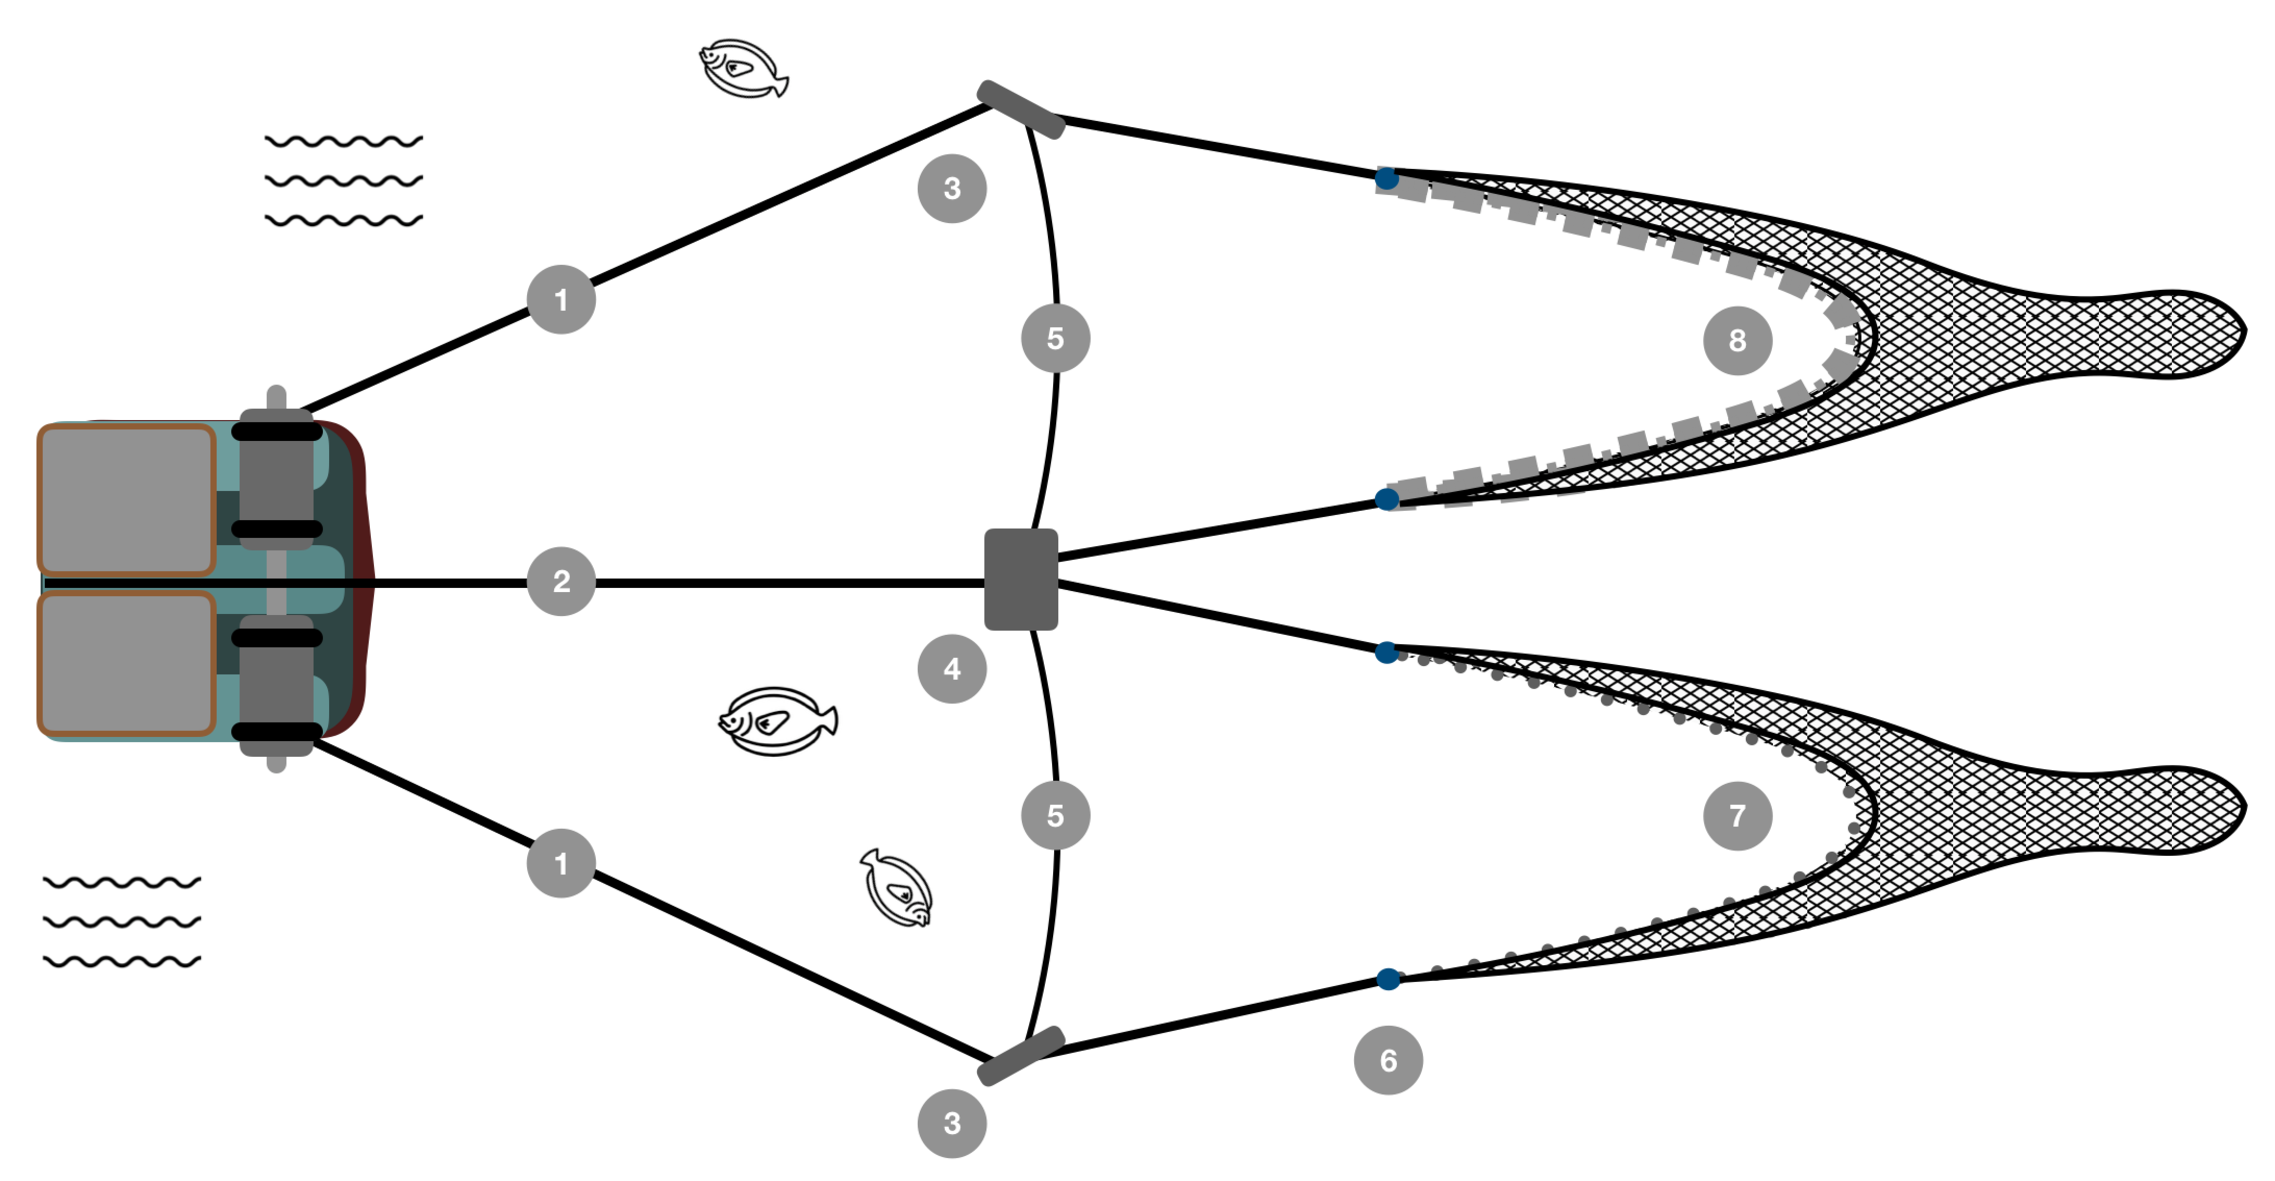
\includegraphics[width = \textwidth]{twin_trawl_diagram.pdf}
\end{center}
\end{figure}

\begin{figure}
\caption{The \textsl{F/V Karen Elizabeth} twin-trawl vessel rigged with rockhopper sweep gear on the right and chain sweep gear on the left.}\label{twin_trawl_photo}
\begin{center}
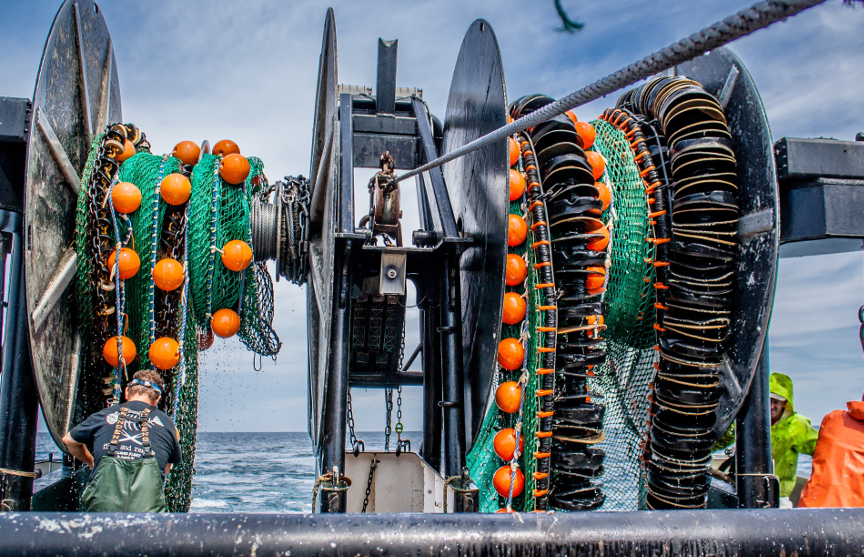
\includegraphics[width = \textwidth]{twin_trawl_photo_small.png}
\end{center}
\end{figure}

\begin{landscape}
\begin{figure}
\caption{Annual locations of stations where the F/V Karen Elizabeth conducted twin-trawl sets with the standard bottom trawl gear and the gear with a chain sweep instead of the rockhopper sweep.}\label{tow_locations}
\begin{center}
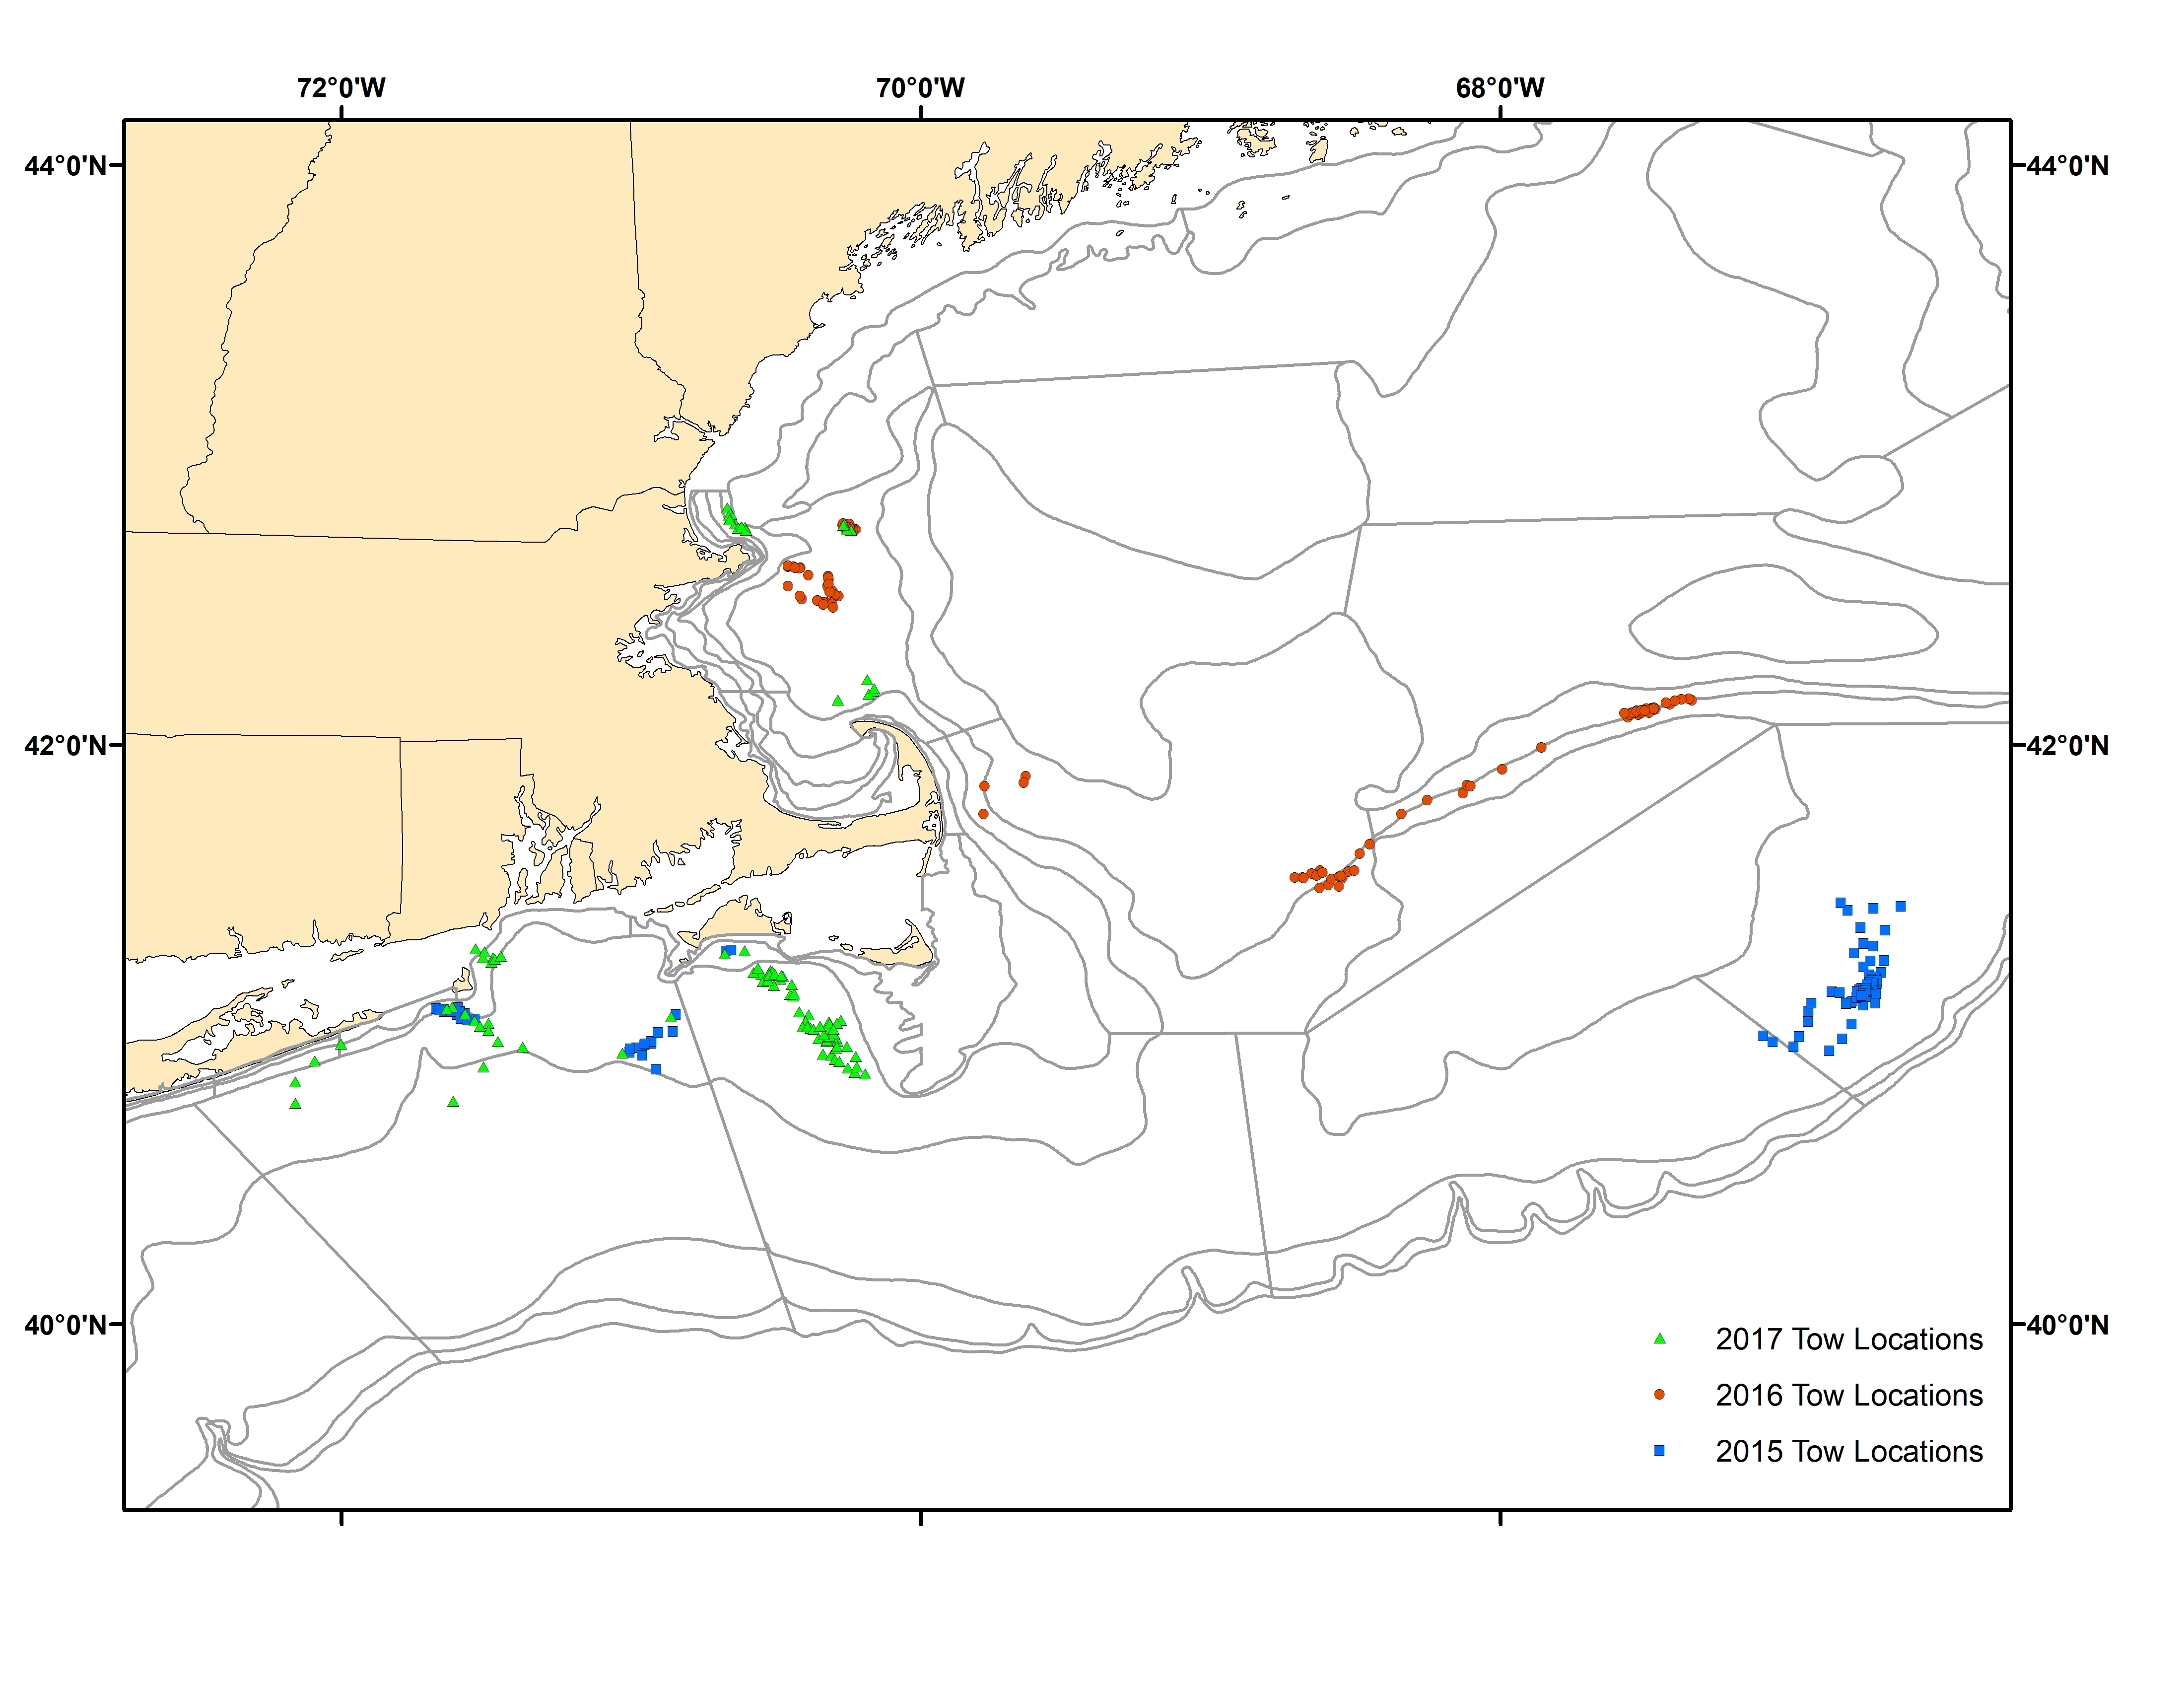
\includegraphics[width = \textwidth]{TwinTrawlLocationsAllYears.jpg}
\end{center}
\end{figure}
\end{landscape}

\clearpage

\begin{figure}
\caption{Relative efficiency  of gears using chain and rockhopper sweeps from the best performing model for each species (Table \ref{best_model_compare}). Blue and red denote results for day and night data, respectively, and thick and thin lines represent overall and paired-tow specific estimates of relative catch efficiency, respectively. There was no diel effect in the best model for American plaice. Points represent empirical estimates of relative efficiency for paired observation by length and paired tow. Polygons and dashed lines represent hessian-based and bootstrap-based 95\% confidence intervals, respectively.}\label{sp_rho_plot}
\begin{center}
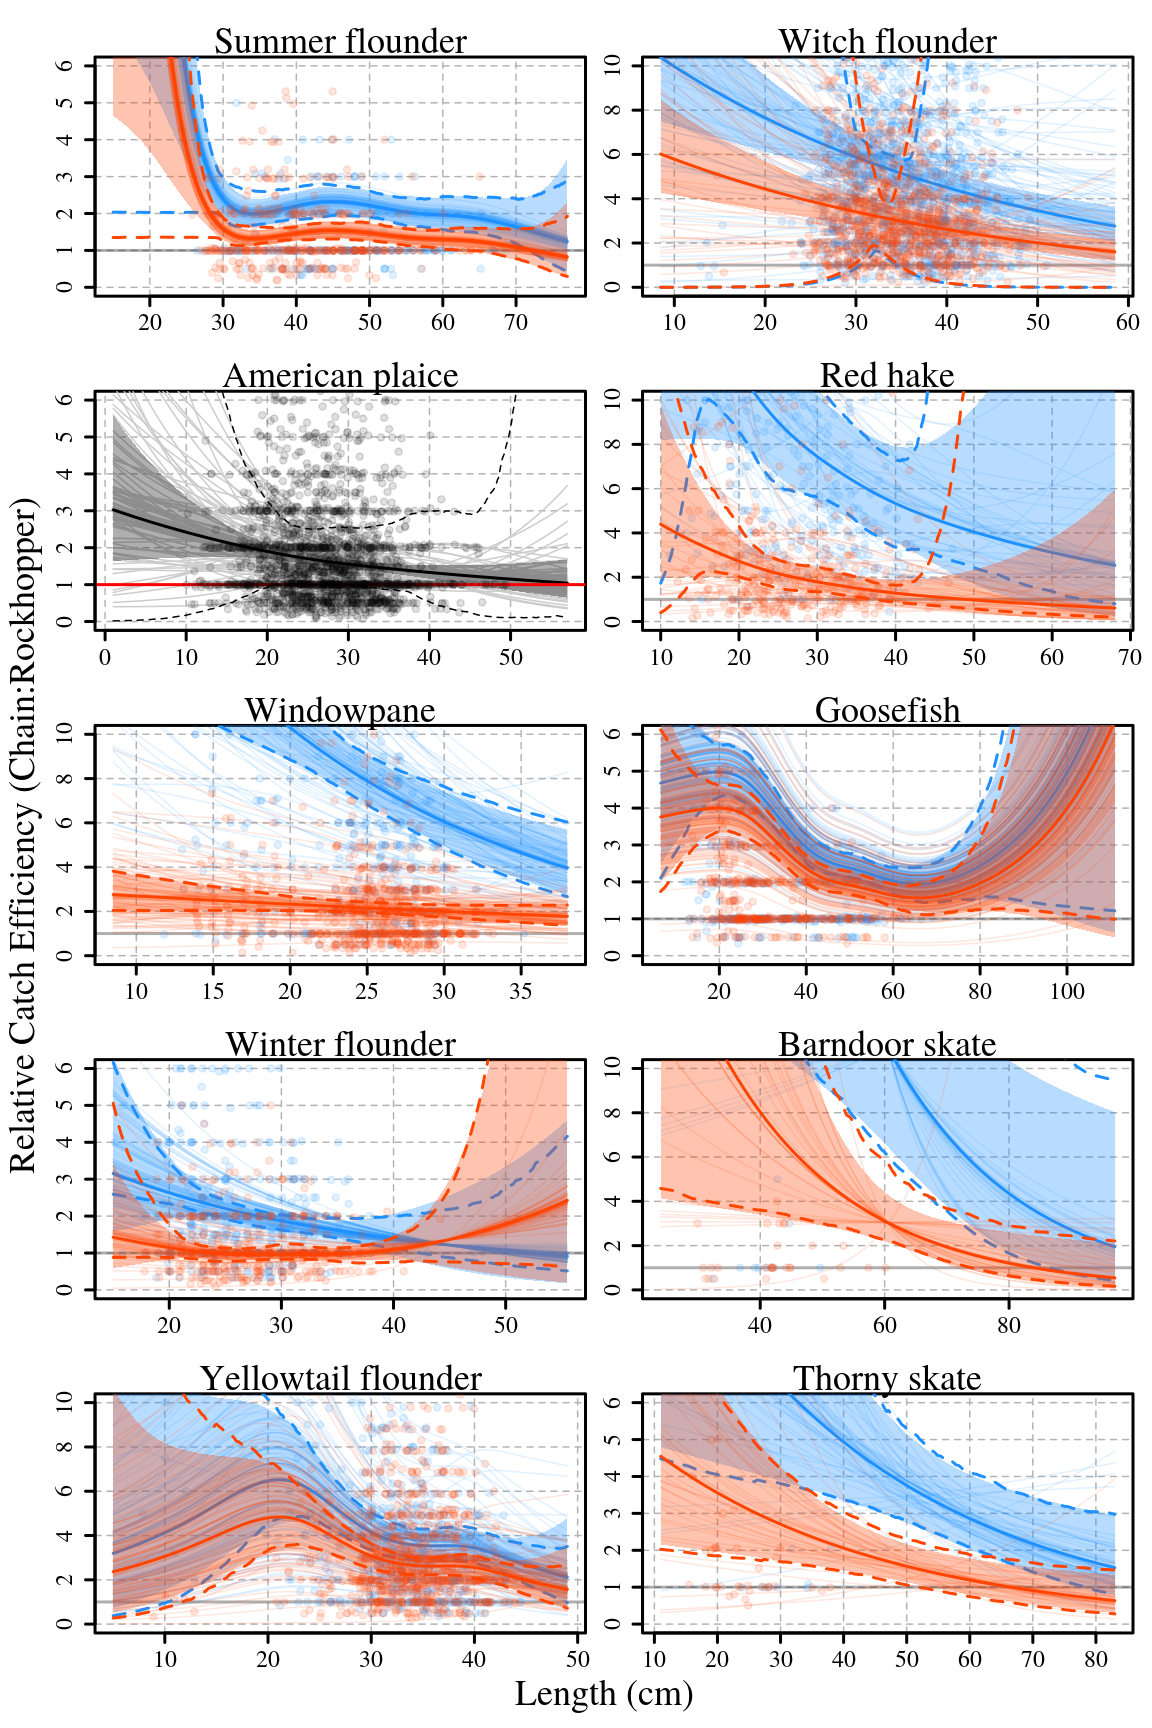
\includegraphics[height = 0.8\textheight]{sp_rho_plot.pdf}
\end{center}
\end{figure}

\clearpage

\begin{figure}
\caption{Annual spring (blue) and fall (red) biomass estimates for each managed stock assuming 100\% efficiency for chain sweep gear with shaded polygons representing bootstrap-based 95\% confidence intervals. Relative catch efficiency at size estimates and bootstraps are from the best performing model for each species (Table \ref{best_model_compare}).}\label{stock_biomass_plot}
\begin{center}
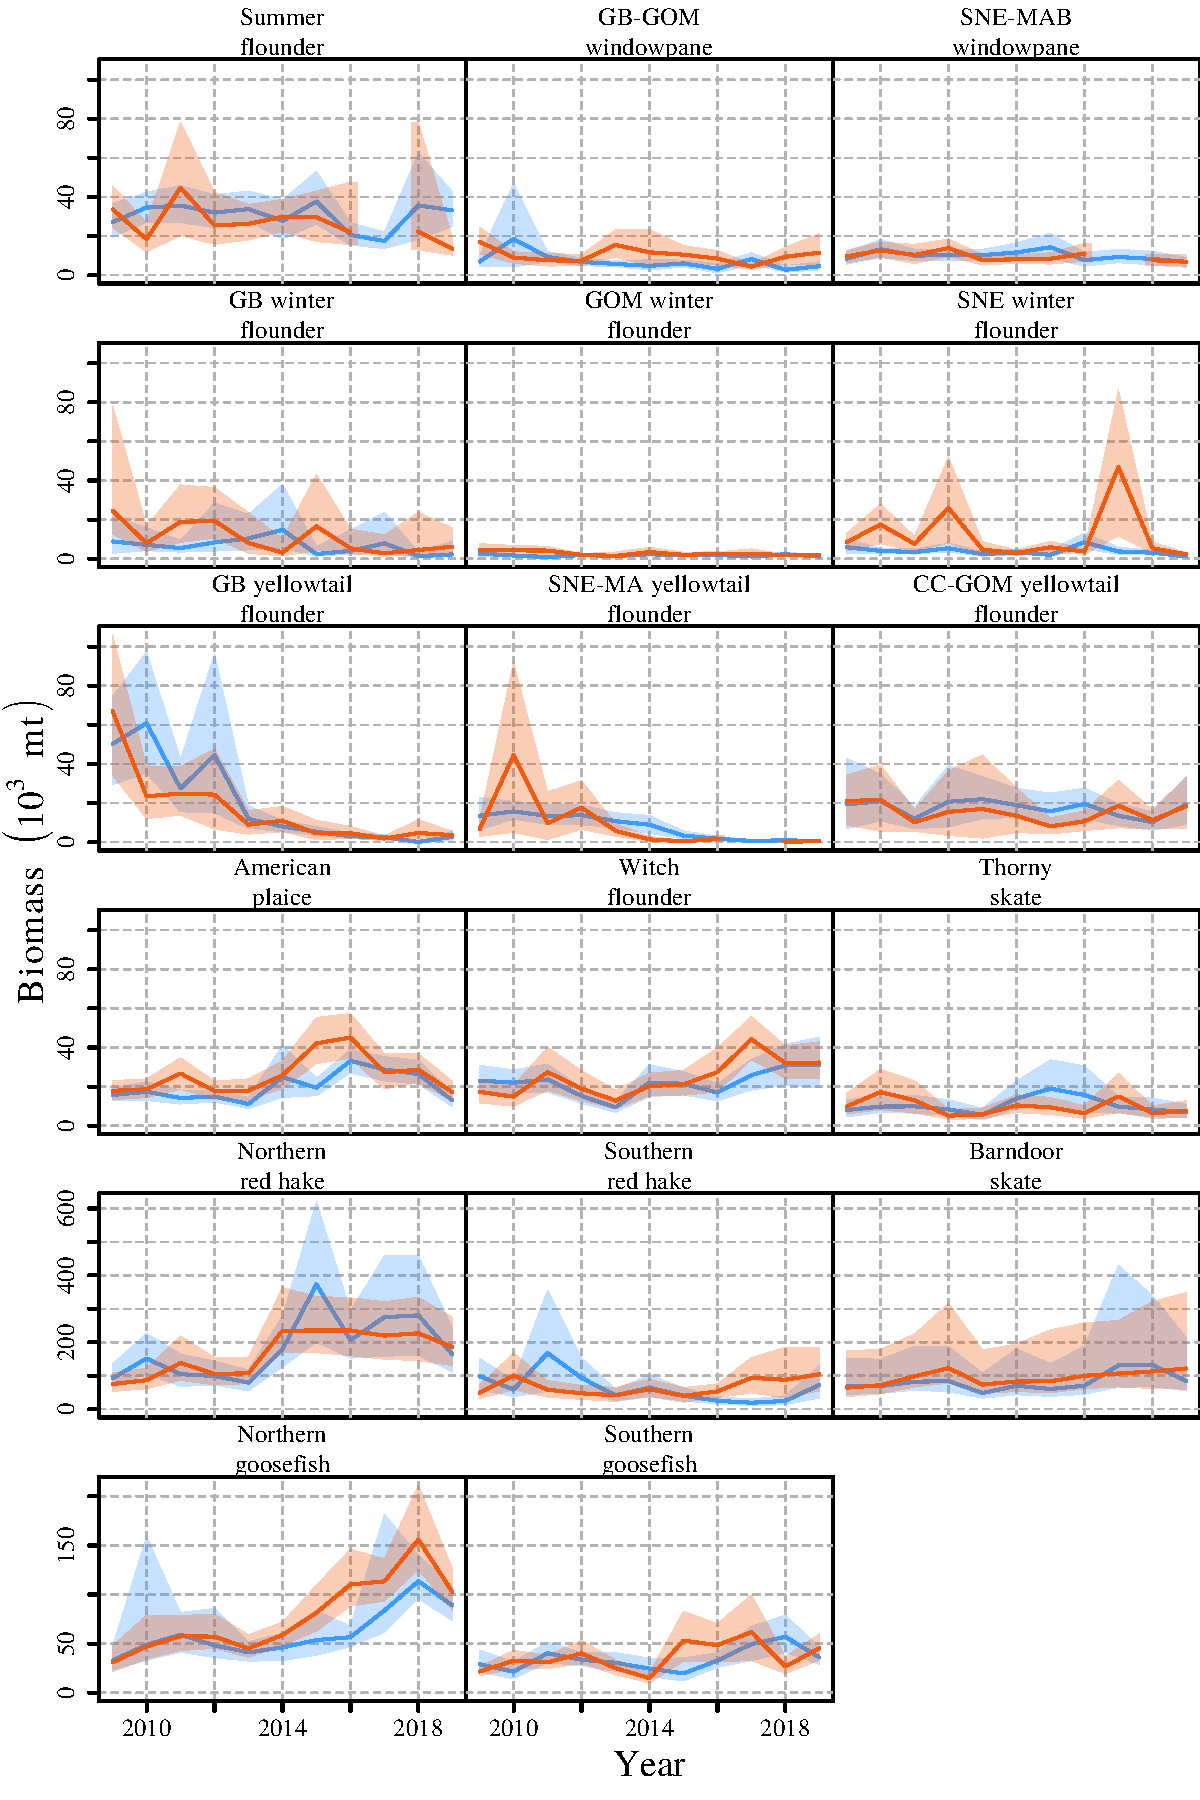
\includegraphics[height = 0.8\textheight]{stock_biomass_plot.pdf}
\end{center}
\end{figure}

\clearpage

\begin{figure}
\caption{Implied catch efficiency of annual spring (blue) and fall (red) bottom trawl survey biomass estimates for each managed stock assuming 100\% efficiency for chain sweep gear with shaded polygons representing bootstrap-based 95\% confidence intervals. Relative catch efficiency at size estimates and bootstraps are from the best performing model for each species (Table \ref{best_model_compare}).}\label{stock_biomass_efficiency_plot}
\begin{center}
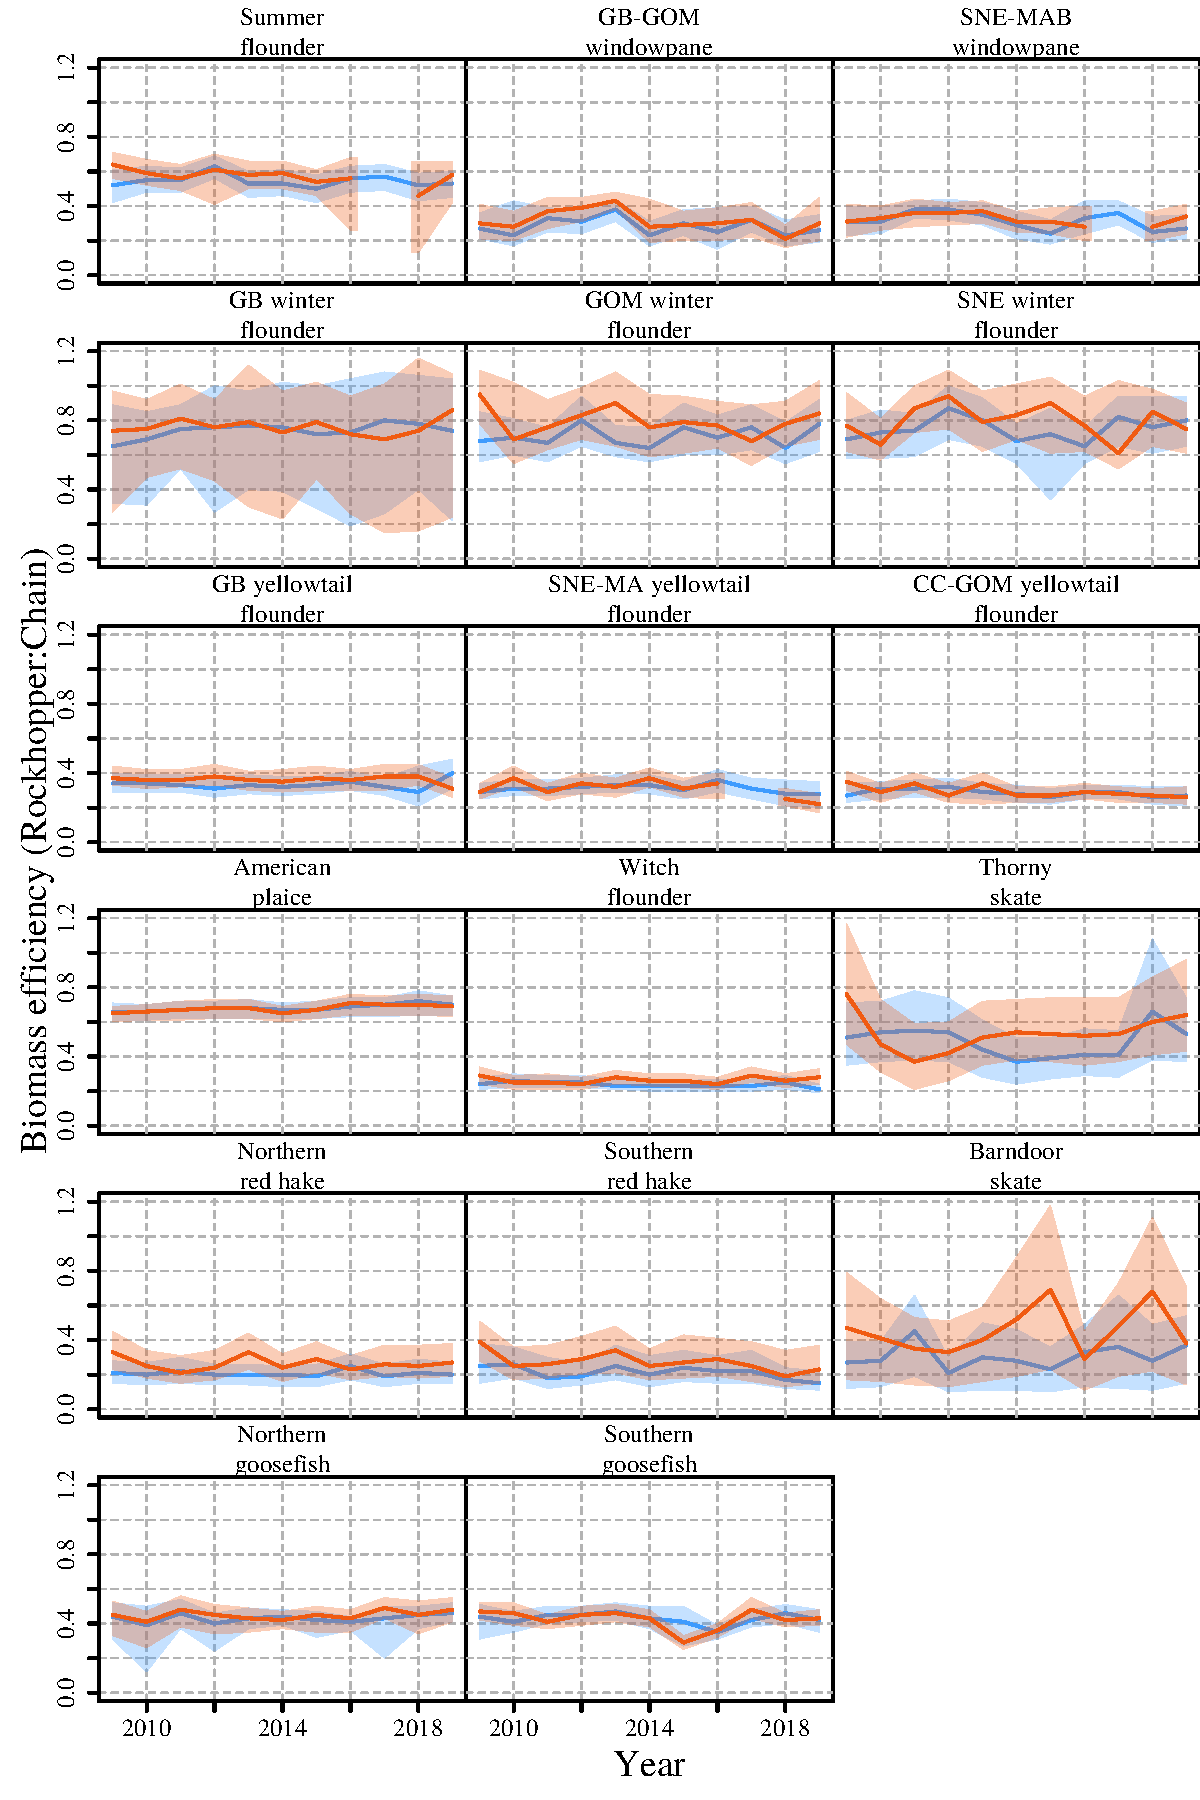
\includegraphics[height = 0.8\textheight]{stock_biomass_efficiency_plot.pdf}
\end{center}
\end{figure}

\clearpage

\begin{table}
\caption{Managed stocks associated with the species for which relative catch efficiency was estimated.}\label{stock_definition_table}
{%latex.default(stock.definition.table, file = paste0("paper/stock_definition_table.tex"),     first.hline.double = FALSE, col.just = rep("l", 2), table.env = FALSE)%
\begin{center}
\begin{tabular}{l}
\hline
\multicolumn{1}{c}{Stock}\tabularnewline
\hline
Summer flounder\tabularnewline
American Plaice\tabularnewline
Georges Bank-Gulf of Maine (GB-GOM) windowpane\tabularnewline
Southern New England-Mid-Atlantic Bight (SNE-MAB) windowpane\tabularnewline
Georges Bank (GB) winter flounder\tabularnewline
Gulf of Maine (GOM) winter flounder\tabularnewline
Southern New England (SNE) winter flounder\tabularnewline
GB yellowtail flounder\tabularnewline
Southern New England-Mid-Atlantic (SNE-MA) yellowtail flounder\tabularnewline
Cape Cod-Gulf of Maine (CC-GOM) yellowtail flounder\tabularnewline
Witch flounder\tabularnewline
Northern red hake\tabularnewline
Southern red hake\tabularnewline
Northern goosefish\tabularnewline
Southern goosefish\tabularnewline
Barndoor skate\tabularnewline
Thorny skate\tabularnewline
\hline
\end{tabular}\end{center}
}
\end{table}

\begin{landscape}
\begin{table}
\caption{Description of relative catch efficiency ($\rho$) and beta-binomial dispersion ($\phi$) parameterizations for binomial and beta-binomial models and number of marginal likelihood parameters ($n_p$) for the 13 base models from \citet{miller13} and fit to paired chain sweep and rockhoppersweep tow data for each species.}\label{base_model_description}
{%latex.default(out, file = paste0(parentdir, "/paper/base_model_description.tex"),     table.env = FALSE, col.just = c("l", "l", "l", "r", "p{0.5\\textwidth}"),     rowname = NULL)%
\begin{center}
\begin{tabular}{lllrp{0.5\textwidth}}
\hline\hline
\multicolumn{1}{c}{Model}&\multicolumn{1}{c}{$\log\left(\rho\right)$}&\multicolumn{1}{c}{$\log\left(\phi\right)$}&\multicolumn{1}{c}{$n_p$}&\multicolumn{1}{c}{Description}\tabularnewline
\hline
BI$_{0}$&$\sim$ 1&--&$ 1$&population-level mean for all observations\tabularnewline
BI$_{1}$&$\sim$ 1 + 1$|$pair&--&$ 2$&population- and random station-level $\rho$\tabularnewline
BI$_{2}$&$\sim$ s(length)&--&$ 3$&population-level smooth size effect on $\rho$\tabularnewline
BI$_{3}$&$\sim$ s(length) + 1$|$pair&--&$ 4$&population-level smooth size effect and random station-level intercept for $\rho$\tabularnewline
BI$_{4}$&$\sim$ s(length) + s(length)$|$pair&--&$ 7$&population-level and random station-level smooth size effects for $\rho$\tabularnewline
BB$_{0}$&$\sim$ 1&$\sim$ 1&$ 2$&population-level $\rho$ and $\phi$\tabularnewline
BB$_{1}$&$\sim$ 1 + 1$|$pair&$\sim$ 1&$ 3$&population-level and random station-level intercept for $\rho$ and population-level $\phi$\tabularnewline
BB$_{2}$&$\sim$ s(length)&$\sim$ 1&$ 4$&population-level smooth size effect on $\rho$ and population-level $\phi$\tabularnewline
BB$_{3}$&$\sim$ s(length)&$\sim$ s(length)&$ 6$&population-level smooth size effect on $\rho$ and $\phi$\tabularnewline
BB$_{4}$&$\sim$ s(length) + 1$|$pair&$\sim$ 1&$ 5$&population-level smooth size effect and random station-level intercept for $\rho$ and population-level $\phi$\tabularnewline
BB$_{5}$&$\sim$ s(length) + 1$|$pair&$\sim$ s(length)&$ 7$&population-level smooth size effect on $\rho$ and $\phi$ and random station-level intercepts for $\rho$\tabularnewline
BB$_{6}$&$\sim$ s(length) + s(length)$|$pair&$\sim$ 1&$ 8$&population-level and random station-level smooth size effects on $\rho$ and population-level $\phi$\tabularnewline
BB$_{7}$&$\sim$ s(length) + s(length)$|$pair&$\sim$ s(length)&$10$&population-level and random station-level smooth size effects on $\rho$ and population-level smooth size effects on $\phi$\tabularnewline
\hline
\end{tabular}\end{center}
}
\end{table}
\end{landscape}

\begin{landscape}
\begin{table}
\caption{Number of paired tows where fish were captured and the number of fish captured and measured for lengths for each species in total and by day or night.}\label{data_table}
{\fontsize{10pt}{10pt}\selectfont%latex.default(nobs.table, file = paste0(parentdir, "/paper/data_table.tex"),     cgroup = c("Paired Tows", "Captured", "\\thead{Both Gears \\\\ Measured}",         "\\thead{Chainsweep \\\\ Measured}", "\\thead{Rockhopper \\\\ Measured}"),     first.hline.double = FALSE, n.cgroup = c(3, 1, 3, 3, 3),     col.just = rep("r", NCOL(nobs.table)), cgroupTexCmd = "normalfont",     rowlabel = "Species", table.env = FALSE)%
\begin{center}
\begin{tabular}{lrrrcrcrrrcrrrcrrr}
\hline
\multicolumn{1}{l}{\normalfont Species}&\multicolumn{3}{c}{\normalfont Paired Tows}&\multicolumn{1}{c}{\normalfont }&\multicolumn{1}{c}{\normalfont Captured}&\multicolumn{1}{c}{\normalfont }&\multicolumn{3}{c}{\normalfont \thead{Both Gears \\ Measured}}&\multicolumn{1}{c}{\normalfont }&\multicolumn{3}{c}{\normalfont \thead{Chainsweep \\ Measured}}&\multicolumn{1}{c}{\normalfont }&\multicolumn{3}{c}{\normalfont \thead{Rockhopper \\ Measured}}\tabularnewline
\cline{2-4} \cline{6-6} \cline{8-10} \cline{12-14} \cline{16-18}
\multicolumn{1}{l}{}&\multicolumn{1}{c}{Total}&\multicolumn{1}{c}{Day}&\multicolumn{1}{c}{Night}&\multicolumn{1}{c}{}&\multicolumn{1}{c}{Total}&\multicolumn{1}{c}{}&\multicolumn{1}{c}{Total}&\multicolumn{1}{c}{Day}&\multicolumn{1}{c}{Night}&\multicolumn{1}{c}{}&\multicolumn{1}{c}{Total}&\multicolumn{1}{c}{Day}&\multicolumn{1}{c}{Night}&\multicolumn{1}{c}{}&\multicolumn{1}{c}{Total}&\multicolumn{1}{c}{Day}&\multicolumn{1}{c}{Night}\tabularnewline
\hline
Summer flounder&141& 75& 66&& 4,154&& 4,154& 1,770& 2,384&& 2,616&1,195&1,421&&1,538&  575&  963\tabularnewline
American plaice&134& 84& 50&&31,983&&19,245&13,619& 5,626&&10,982&7,775&3,207&&8,263&5,844&2,419\tabularnewline
Windowpane&195&100& 95&&15,310&&13,014& 6,221& 6,793&& 9,854&5,443&4,411&&3,160&  778&2,382\tabularnewline
Winter flounder&171& 97& 74&& 6,586&& 6,449& 3,605& 2,844&& 3,805&2,385&1,420&&2,644&1,220&1,424\tabularnewline
Yellowtail flounder&192&101& 91&&18,545&&14,134& 6,849& 7,285&&10,065&5,297&4,768&&4,069&1,552&2,517\tabularnewline
Witch flounder&132& 83& 49&&57,133&&23,927&13,899&10,028&&14,899&9,271&5,628&&9,028&4,628&4,400\tabularnewline
Red hake& 73& 40& 33&&47,275&&12,585& 6,614& 5,971&& 8,587&4,908&3,679&&3,998&1,706&2,292\tabularnewline
Goosefish&302&165&137&& 8,798&& 8,541& 3,985& 4,556&& 6,409&3,053&3,356&&2,132&  932&1,200\tabularnewline
Barndoor skate& 62& 33& 29&&   502&&   502&   219&   283&&   397&  198&  199&&  105&   21&   84\tabularnewline
Thorny skate& 90& 56& 34&&   907&&   907&   399&   508&&   648&  311&  337&&  259&   88&  171\tabularnewline
\hline
\end{tabular}\end{center}
}
\end{table}
\end{landscape}

\begin{landscape}
\begin{table}\caption{Difference in AIC for each of the 13 models described in Table \ref{base_model_description} from the best model ($\bf 0$) by species.}\label{base_model_compare}
{%latex.default(x, file = paste0(parentdir, "/paper/base_model_compare.tex"),     col.just = rep("r", NCOL(x)), numeric.dollar = FALSE, cellTexCmds = cell.format,     rowlabel = "", table.env = FALSE)%
\begin{center}
\begin{tabular}{lrrrrrrrrrrrrr}
\hline\hline
\multicolumn{1}{l}{}&\multicolumn{1}{c}{BI$_{0}$}&\multicolumn{1}{c}{BI$_{1}$}&\multicolumn{1}{c}{BI$_{2}$}&\multicolumn{1}{c}{BI$_{3}$}&\multicolumn{1}{c}{BI$_{4}$}&\multicolumn{1}{c}{BB$_{0}$}&\multicolumn{1}{c}{BB$_{1}$}&\multicolumn{1}{c}{BB$_{2}$}&\multicolumn{1}{c}{BB$_{3}$}&\multicolumn{1}{c}{BB$_{4}$}&\multicolumn{1}{c}{BB$_{5}$}&\multicolumn{1}{c}{BB$_{6}$}&\multicolumn{1}{c}{BB$_{7}$}\tabularnewline
\hline
   Summer flounder&   27.96&   13.53&   8.9&\bfseries   0&   &   28.64&   15.45&   10.59&   &   &   &   &   \tabularnewline
   American plaice&   821.11&   546.54&   743.34&   494.92&   415.63&   179.48&   71.76&   141.44&   &   37.06&   &   0.71&\bfseries   0\tabularnewline
   Windowpane&   1045.06&   38.51&   1029.72&   17.03&\bfseries   0&   585.7&   32.22&   572.73&   &   15.27&   &   &   \tabularnewline
   Winter flounder&   216.47&   15.73&   200.33&   3.02&\bfseries   0&   163.31&   16.63&   151.66&   151.01&   4.21&   6.78&   1.41&   \tabularnewline
   Yellowtail flounder&   727.15&   97.93&   727.36&   51.84&   10.96&   394.94&   70.2&   391.13&   371.13&   31.85&   &\bfseries   0&   3.33\tabularnewline
   Witch flounder&   1424.17&   212.64&   1372.66&   &   35.33&   881.28&   142.53&   844.47&   &   81.37&   &\bfseries   0&   \tabularnewline
   Red hake&   1884.51&   295.85&   1697.48&   170.75&   &   627.33&   166.43&   590.92&   &   95.8&   59.31&\bfseries   0&   0.83\tabularnewline
   Goosefish&   227.67&   87.23&   80.37&\bfseries   0&   &   219.13&   &   76.54&   &   &   &   &   \tabularnewline
   Barndoor skate&   36.51&   10.01&   31.34&   2.72&\bfseries   0&   36.23&   11.99&   29.03&   &   4.6&   &   &   \tabularnewline
   Thorny skate&   39.04&   8.57&   32.65&   3.44&   1.15&   22.38&   5.84&   18.66&   &   1.38&   5.19&\bfseries   0&   \tabularnewline
\hline
\end{tabular}\end{center}
}
\end{table}
\end{landscape}

\begin{landscape}
\begin{table}\caption{Best performing models from Table \ref{base_model_compare} and extended models that include diel effects on relative catch efficiency for each species with the number of parameters for each model ($n_p$) and the differences in AIC ($\Delta$AIC) from the best of the three models ($\bf 0$) by species.}\label{best_model_compare}
{\fontsize{7pt}{7pt}\selectfont%latex.default(temp, file = paste0(parentdir, "/paper/best_model_compare.tex"),     rgroup = sp.info$sp.pretty.names[ind], n.rgroup = rep(3,         length(ind)), col.just = c("l", "l", "l", rep("r", 2)),     numeric.dollar = FALSE, cellTexCmds = cell.format, rowlabel = "",     rowname = rep("", NROW(temp)), table.env = FALSE)%
\begin{center}
\begin{tabular}{llllrr}
\hline\hline
\multicolumn{1}{l}{}&\multicolumn{1}{c}{Model}&\multicolumn{1}{c}{$\log\left(\rho\right)$}&\multicolumn{1}{c}{$\log\left(\phi\right)$}&\multicolumn{1}{c}{$n_p$}&\multicolumn{1}{c}{$\Delta$AIC}\tabularnewline
\hline
{\bfseries Summer flounder}&&&&&\tabularnewline
   ~~&   BI$_{3}$&   $\sim$ s(length) + 1$|$pair&   --&    4&   22.92\tabularnewline
   ~~&   BI$_{3a}$&   $\sim$ dn + s(length) + 1$|$pair&   --&    5&\bfseries   0\tabularnewline
   ~~&   BI$_{3b}$&   $\sim$ dn * s(length) + 1$|$pair&   --&    7&   1.74\tabularnewline
\hline
{\bfseries American plaice}&&&&&\tabularnewline
   ~~&   BB$_{7}$&   $\sim$ s(length) + s(length)$|$pair&   $\sim$ s(length)&   10&\bfseries   0\tabularnewline
   ~~&   BB$_{7a}$&   $\sim$ dn + s(length) + s(length)$|$pair&   $\sim$ s(length)&   11&   1.43\tabularnewline
   ~~&   BB$_{7b}$&   $\sim$ dn * s(length) + s(length)$|$pair&   $\sim$ s(length)&   13&   2.95\tabularnewline
\hline
{\bfseries Windowpane}&&&&&\tabularnewline
   ~~&   BI$_{4}$&   $\sim$ s(length) + s(length)$|$pair&   --&    7&   152.1\tabularnewline
   ~~&   BI$_{4a}$&   $\sim$ dn + length + s(length)$|$pair&   --&    7&   4.06\tabularnewline
   ~~&   BI$_{4b}$&   $\sim$ dn * length + s(length)$|$pair&   --&    8&\bfseries   0\tabularnewline
\hline
{\bfseries Winter flounder}&&&&&\tabularnewline
   ~~&   BI$_{4}$&   $\sim$ s(length) + s(length)$|$pair&   --&    7&   50.68\tabularnewline
   ~~&   BI$_{4a}$&   $\sim$ dn + s(length) + length$|$pair&   --&    7&   0.3\tabularnewline
   ~~&   BI$_{4b}$&   $\sim$ dn * s(length) + length$|$pair&   --&    9&\bfseries   0\tabularnewline
\hline
{\bfseries Yellowtail flounder}&&&&&\tabularnewline
   ~~&   BB$_{6}$&   $\sim$ s(length) + s(length)$|$pair&   $\sim$ 1&    8&   3.84\tabularnewline
   ~~&   BB$_{6a}$&   $\sim$ dn + s(length) + s(length)$|$pair&   $\sim$ 1&    9&\bfseries   0\tabularnewline
   ~~&   BB$_{6b}$&   $\sim$ dn * s(length) + s(length)$|$pair&   $\sim$ 1&   11&   3.48\tabularnewline
\hline
{\bfseries Witch flounder}&&&&&\tabularnewline
   ~~&   BB$_{6}$&   $\sim$ s(length) + s(length)$|$pair&   $\sim$ 1&    8&   19.68\tabularnewline
   ~~&   BB$_{6a}$&   $\sim$ dn + length + s(length)$|$pair&   $\sim$ 1&    8&\bfseries   0\tabularnewline
   ~~&   BB$_{6b}$&   $\sim$ dn * length + s(length)$|$pair&   $\sim$ 1&    9&   1.52\tabularnewline
\hline
{\bfseries Red hake}&&&&&\tabularnewline
   ~~&   BB$_{6}$&   $\sim$ s(length) + s(length)$|$pair&   $\sim$ 1&    8&   32.35\tabularnewline
   ~~&   BB$_{6a}$&   $\sim$ dn + s(length) + s(length)$|$pair&   $\sim$ 1&    8&\bfseries   0\tabularnewline
   ~~&   BB$_{6b}$&   $\sim$ dn * s(length) + s(length)$|$pair&   $\sim$ 1&   10&   3.18\tabularnewline
\hline
{\bfseries Goosefish}&&&&&\tabularnewline
   ~~&   BI$_{3}$&   $\sim$ s(length) + 1$|$pair&   --&    4&   5.44\tabularnewline
   ~~&   BI$_{3a}$&   $\sim$ dn + s(length) + 1$|$pair&   --&    5&\bfseries   0\tabularnewline
   ~~&   BI$_{3b}$&   $\sim$ dn * s(length) + 1$|$pair&   --&    7&   6.8\tabularnewline
\hline
{\bfseries Barndoor skate}&&&&&\tabularnewline
   ~~&   BI$_{4}$&   $\sim$ s(length) + s(length)$|$pair&   --&    7&   15.57\tabularnewline
   ~~&   BI$_{4a}$&   $\sim$ dn + length + length$|$pair&   --&    5&\bfseries   0\tabularnewline
   ~~&   BI$_{4b}$&   $\sim$ dn * length + length$|$pair&   --&    6&   1.83\tabularnewline
\hline
{\bfseries Thorny skate}&&&&&\tabularnewline
   ~~&   BB$_{6}$&   $\sim$ s(length) + s(length)$|$pair&   $\sim$ 1&    8&   15.51\tabularnewline
   ~~&   BB$_{6a}$&   $\sim$ dn + length + length$|$pair&   $\sim$ 1&    7&\bfseries   0\tabularnewline
   ~~&   BB$_{6b}$&   $\sim$ dn * length + length$|$pair&   $\sim$ 1&    8&   1.38\tabularnewline
\hline
\end{tabular}\end{center}
}
\end{table}
\end{landscape}

\begin{table}
\caption{Average of annual (2009-2019) ratios of coefficients of variation for calibrated and uncalibrated biomass indices for each stock by seasonal survey. Coefficients of variation are based on bootstrap resampling of paired tow observations, survey station data and associated length and weight observations. Annual indices for fall 2017 were not available for summer flounder, SNE-MA windowpane, and SNE-MA yellowtail flounder.}\label{stock_cv_ratios}
{%latex.default(round(cv.ratios[stock.order, 2:1], 2), file = paste0(parentdir,     "/paper/stock_cv_ratios.tex"), cgroup = c("\\thead{Average CV Ratio \\\\ Calibrated:Uncalibrated}"),     first.hline.double = FALSE, n.cgroup = 2, collabel.just = rep("r",         2), col.just = rep("r", 2), cgroupTexCmd = "normalfont",     rowlabel = "Stock", table.env = FALSE)%
\begin{center}
\begin{tabular}{lrr}
\hline
\multicolumn{1}{l}{\normalfont Stock}&\multicolumn{2}{c}{\normalfont \thead{Average CV Ratio \\ Calibrated:Uncalibrated}}\tabularnewline
\cline{2-3}
\multicolumn{1}{l}{}&\multicolumn{1}{r}{Spring}&\multicolumn{1}{r}{Fall}\tabularnewline
\hline
Summer flounder&$1.13$&$1.51$\tabularnewline
American plaice&$1.07$&$1.02$\tabularnewline
GB-GOM windowpane&$1.03$&$1.07$\tabularnewline
SNE-MAB windowpane&$1.06$&$0.90$\tabularnewline
GB winter flounder&$3.19$&$3.89$\tabularnewline
GOM winter flounder&$1.05$&$1.07$\tabularnewline
SNE winter flounder&$1.77$&$0.99$\tabularnewline
GB yellowtail flounder&$1.06$&$0.98$\tabularnewline
SNE-MA yellowtail flounder&$1.05$&$0.99$\tabularnewline
CC-GOM yellowtail flounder&$1.01$&$1.02$\tabularnewline
Witch flounder&$1.12$&$1.11$\tabularnewline
Northern red hake&$1.95$&$2.78$\tabularnewline
Southern red hake&$1.28$&$1.28$\tabularnewline
Northern goosefish&$1.93$&$1.34$\tabularnewline
Southern goosefish&$1.18$&$1.04$\tabularnewline
Barndoor skate&$2.47$&$2.78$\tabularnewline
Thorny skate&$1.14$&$1.20$\tabularnewline
\hline
\end{tabular}\end{center}
}
\end{table}

\begin{table}
\caption{Average correlation of annual (2009-2019) calibrated biomass indices for each stock by seasonal survey. Annual indices for fall 2017 were not available for SNE-MA windowpane and SNE-MA yellowtail flounder.}\label{stock_mean_cor}
{%latex.default(round(mean.cor[stock.order, c(3, 1)], 2), file = paste0(parentdir,     "/paper/stock_mean_cor.tex"), first.hline.double = FALSE,     n.cgroup = 2, colheads = c("Spring", "Fall"), rowlabel = "Stock",     table.env = FALSE)%
\begin{center}
\begin{tabular}{lrr}
\hline
\multicolumn{1}{l}{Stock}&\multicolumn{1}{c}{Spring}&\multicolumn{1}{c}{Fall}\tabularnewline
\hline
Summer flounder&$0.16$&$0.14$\tabularnewline
American plaice&$0.09$&$0.06$\tabularnewline
GB-GOM windowpane&$0.06$&$0.04$\tabularnewline
SNE-MAB windowpane&$0.06$&$0.05$\tabularnewline
GB winter flounder&$0.65$&$0.45$\tabularnewline
GOM winter flounder&$0.05$&$0.05$\tabularnewline
SNE winter flounder&$0.07$&$0.03$\tabularnewline
GB yellowtail flounder&$0.05$&$0.04$\tabularnewline
SNE-MA yellowtail flounder&$0.07$&$0.02$\tabularnewline
CC-GOM yellowtail flounder&$0.05$&$0.04$\tabularnewline
Witch flounder&$0.10$&$0.10$\tabularnewline
Northern red hake&$0.42$&$0.34$\tabularnewline
Southern red hake&$0.25$&$0.21$\tabularnewline
Northern goosefish&$0.21$&$0.30$\tabularnewline
Southern goosefish&$0.10$&$0.07$\tabularnewline
Barndoor skate&$0.74$&$0.81$\tabularnewline
Thorny skate&$0.29$&$0.25$\tabularnewline
\hline
\end{tabular}\end{center}
}
\end{table}

\end{document}
